%%%%%%%%%%%%%%%%%%%%%%%%%%%%%%%%%%%%%%%%%%%%%%%%%%%%%%%%%%%%%%%%%%%%%%%%%%%%%%%%%%%%%%%%%%%%%
%%									Chapitre 2												%
%%%%%%%%%%%%%%%%%%%%%%%%%%%%%%%%%%%%%%%%%%%%%%%%%%%%%%%%%%%%%%%%%%%%%%%%%%%%%%%%%%%%%%%%%%%%%

\chapter{Détection de Nouveauté}
	\citationChap{
		D'abord, j'observe les êtres humains car je les aime bien. J'enregistre dans ma tête tout ce que j'ai remarqué, et ensuite, avec les souvenirs de ce que j'ai vu, je dessine.
	}{Hayao Miyazaki}
	\minitoc
	\newpage

%%%%%%%%%%%%%%%%%%%%%%%%%%%%%%%%%%%%%%%%%%%%%%%%%%%%%%%%%%%%%%%%%%%%%%%%%%%%%%%%%%%%%%%%%%%%%



% Début du chapitre
			
	\section{Introduction}

	\section{Application aux images}\label{sec:images}

	Il existe de nombreuses possibilités différentes pour apprendre des images avec la quantification vectorielle, dû au grand nombre de façons de découper une image en vecteurs d'entrée. Pour présenter l'impact que peut avoir ce découpage, on peut considérer deux extrêmes : apprendre l'image en entier ou apprendre chaque pixel individuellement. Le premier cas peut sembler absurde dans le cas d'une seule image (une base de données d'un seul élément), mais peut présenter un intérêt lorsque l'on considère une suite d'images par exemple. Dans cet exemple, l'environnement appris serait défini par l'entièreté de ce que voit le capteur et tous les changements, où qu'ils soient dans l'image, auraient de l'importance.

	Le second extrême est l'apprentissage au niveau du pixel. Dans cette approche on prend chaque pixel individuel comme un vecteur d'entrée, ce qui rendrait l'espace d'entrée unidimensionnel pour une image en niveau de gris (ou tridimensionnel si l'image est en couleur, plus de détails dans la section \ref{sec:img:colors}). Sur un plan conceptuel, ce choix considère qu'une image est définie uniquement par les couleurs ou luminosités présentes, peu importe leur positions dans celle-ci. C'est utilisé notamment dans la détection de changements dans la littérature [réf]. Il existe un très grand nombre d'autres découpages possibles entre ces deux extrêmes, chacun représentant une certaine façon de conceptualiser une image et définissant la notion de nouveauté. Celle-ci étant un changement à un quelconque endroit de l'image dans le premier cas, et l'apparition d'une nouvelle couleur dans l'image dans le second.

	Il est important donc de considérer le contexte de nos travaux pour définir la façon de représenter une image, notre application étant la detection de nouveauté. Dans ce contexte, nous considérons qu'une image est une combinaison de nombreux éléments plus petits. Par exemple, une photographie d'un lac de montagne \ref{fig:img:nino} peut être décrite comme étant la combinaison d'un élément de lac (avec sa couleur, bleu sombre et sa texture uniforme), d'un élément de plaine herbeuse (verte et uniforme), d'éléments rocailleux qui sont gris et soit uniformes (dans le premier plan) soit plus contrastés en se combinant avec la verdure de la végétation (dans les bords de l'image), et ainsi de suite. Ce découpage "sémantique" de l'image est ce qui permet la détection de nouveauté  de fonctionner, car dans notre cas la nouveauté est par définition ce qui n'est pas déjà dans l'image et donc ne faisant pas partie de ces classes d'éléments. Pour regrouper les parties d'une images appartenant au même élément, il est nécessaire d'avoir une information mise en contexte (un pixel seul ne suffit généralement pas à savoir à quel élément il appartient dans l'image), ce qui implique que les pixels doivent être pris dans leurs environnements locaux pour conserver l'information de voisinage comme la texture par exemple. Nous avons donc choisi de découper l'image en plus petites images à la façon d'une mosaique, que nous appellerons des imagettes. Ces imagettes (d'une taille arbitraire en hauteur et largeur) conservent l'environnement local tout en étant suffisament petites pour être précises dans l'espace. Une imagette ne représentant qu'une partie d'un élément et non pas regroupant plusieurs éléments, ce qui réduirait sa capacité de généralisation [détailler ce point ?]. Mais aussi permettent d'avoir une base d'apprentissage assez étoffée pour tirer parti des propriétés de nos modèles de quantification vectorielle et de leur topologie. La partie pratique de l'apprentissage d'une image, sa représentation et sa reconstruction sont abordés dans la section suivante \ref{sec:img:compression}.


	\begin{figureth}
		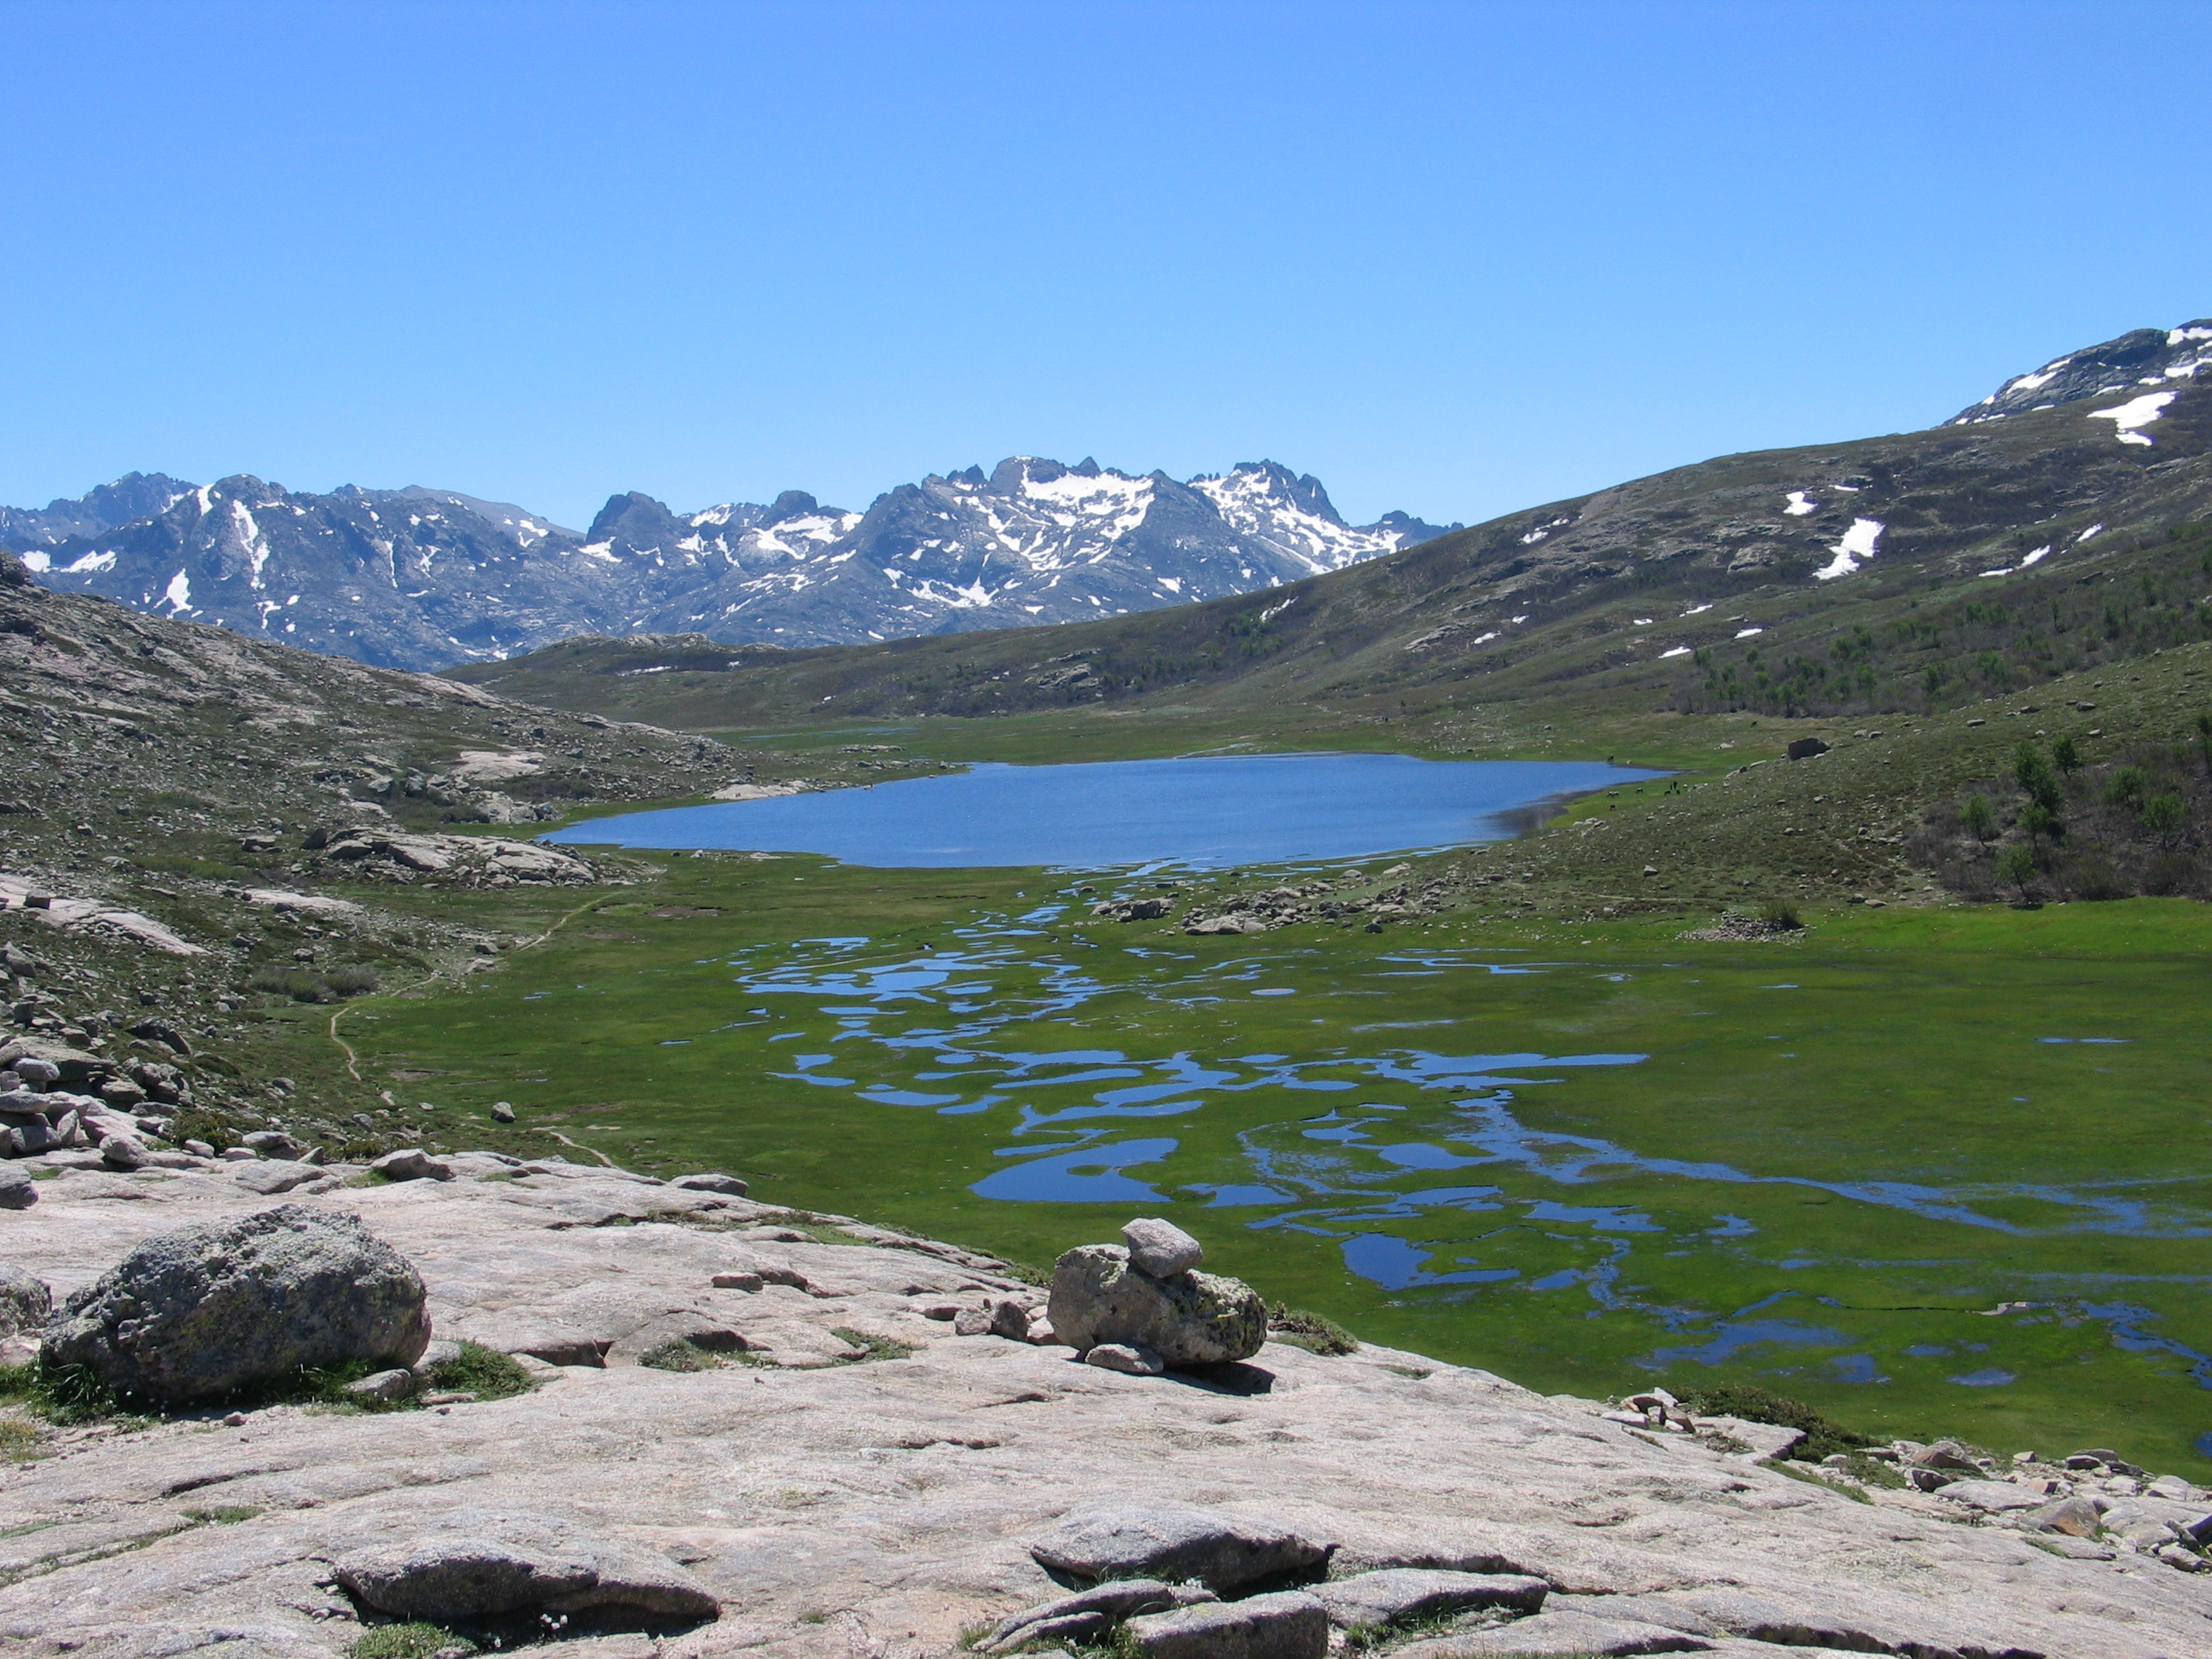
\includegraphics[width=\linewidth]{Lac_de_Nino}
		\caption[Lac de Nino]{Exemple d'image comportant plusieurs éléments notables tels qu'un lac (bleu sombre et uniforme), une plaine herbeuse (verte et uniforme), d'éléments rocailleux qui sont gris et soit uniformes (dans le premier plan) soit plus contrastés en se combinant avec la verdure de la végétation (dans les bords de l'image), et ainsi de suite.[Modifier la figure]}\label{fig:img:nino}
	\end{figureth}

	\subsection{Apprentissage et reconstruction}\label{sec:img:compression}
	\subsubsection{Apprentissage}
	La première étape nécessaire à l'apprentissage est la constitution de la base d'apprentissage à partir de l'image. L'utilisation de modèles de quantification vectorielle établissent la première contrainte pour le découpage : les imagettes doivent être d'une taille fixe. En effet il est nécessaire pour les SOM comme pour les GNG et leurs variantes que tous les vecteurs d'entrées soient de la même longueur pour que le calcul de distance avec les neurones fonctione, qu'ils représentent le plus fidèlement possible les entrées qui leurs sont attachées.

	Nous avons également choisi de limiter nos tailles d'imagettes à des carrés, avec la hauteur égale à la longeur, pour des raisons de simplicité. Il est possible que des imagettes plus larges que hautes ou plus hautes que larges représentent mieux les éléments de l'image que l'on apprend. Cependant ce serait une préférence spécifique à chaque image et peu généralisable, car si on effectue par exemple une rotation de 90° de l'image, la préférence s'inversera. L'inversement des tailles dans les imagettes carrées ne changeant rien, elles sont pour leur part insensibles aux rotations discrètes de l'image (par pas de 90°).

	Dans la version classique \cite{amerijckx-compression}, le découpage de l'image se fait en mosaique, sans superpositions entre les imagettes. C'est à dire que chaque pixel n'appartient qu'à une seule imagette. Le processus est montré sur la figure \ref{fig:img:rep} Si les dimensions de l'images ne sont pas un multiple de la taille des imagettes, les pixels en trop sont rognés par la droite et par le bas [possible de centrer et de rogner tous les côtés en même temps], car en général les bords ne contiennent pas beaucoup d'informations.

	\begin{figureth}
		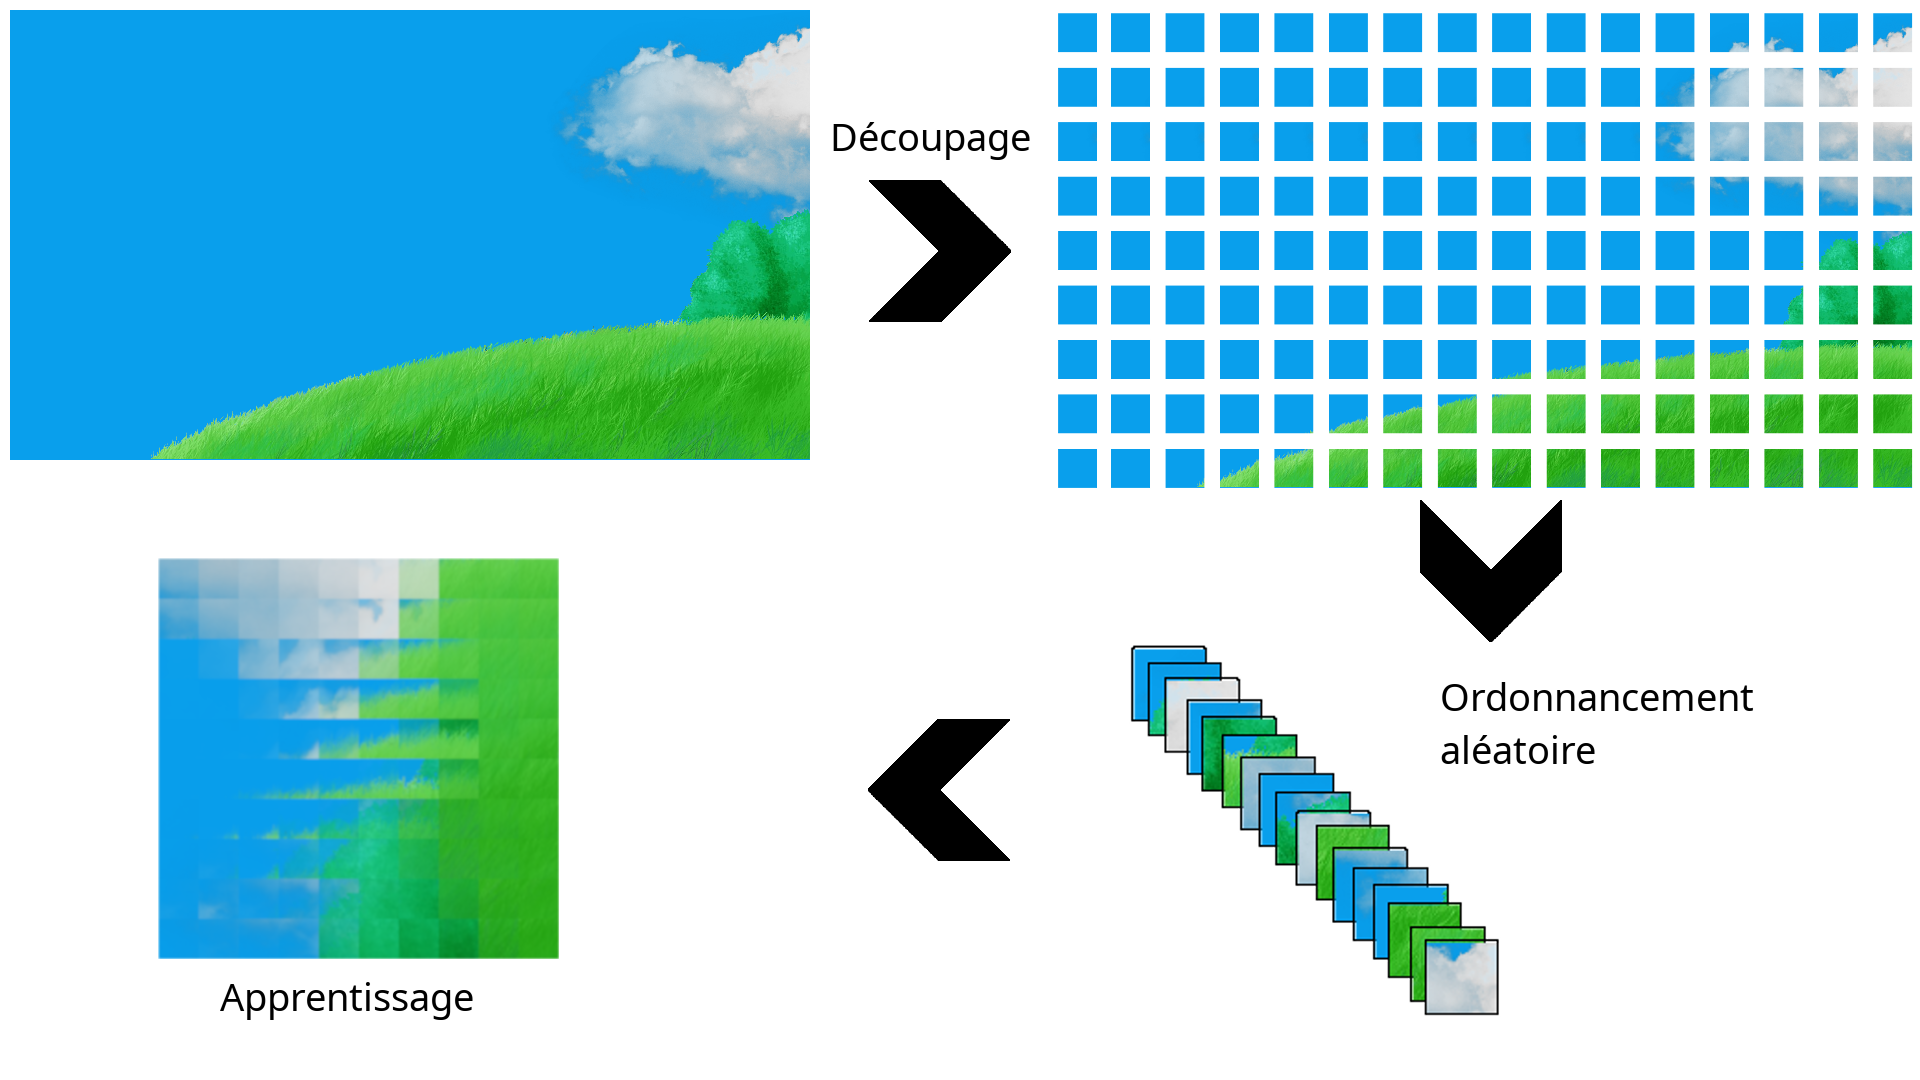
\includegraphics[width=\linewidth]{image_representation}
		\caption[Représentation d'une image]{Illustration du processus de représentation et d'apprentissage d'une image par une SOM.}\label{fig:img:rep}
	\end{figureth}

	\subsubsection{Reconstruction}

	Une fois l'apprentissage terminé, il y a deux résultats. Le premier est le modèle entrainé avec les différents poids des neurones codant une imagette représentante du cluster d'imagettes associé à ce neurone. Le second est la liste pour chaque imagette de l'image l'indexe du neurone le plus proche de celle-ci, qui pourra être utilisée pour la reconstruction de l'image d'apprentissage.  

	Pour reconstruire une image à partir de la liste des indexes de BMU, il suffit de remplacer chaque index par le vecteur prototype du neurone auquel il correspond. Ces vecteurs prototypes devront être réassemblés en imagettes (dans un tableau à 2 dimensions à la place d'un vecteur à une dimension), et placées à la bonne position pour reformer l'image.

	Il est aussi possible de reconstruire une image qui n'a pas été apprise. Pour cela il faut créer la liste d'indexes de neurones des imagettes de la nouvelle image, et de reconstruire ensuite l'image par le même procédé que montré précédemment. Il faut noter que l'image que l'on souhaite reconstituer doit être proche de l'image apprise pour obtenir un résultat correct.

	\begin{figureth}
		\begin{subfigureth}{\textwidth}
			\includegraphics[width=\linewidth]{triangle/Image_compression2}
		\end{subfigureth}
		\begin{subfigureth}{\textwidth}
			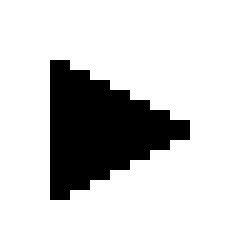
\includegraphics[width=0.2\linewidth]{triangle/triangle_original}\hfill
			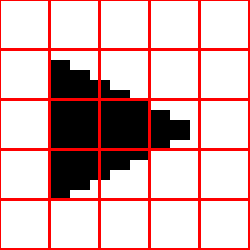
\includegraphics[width=0.2\linewidth]{triangle/triangle_grid}\hfill
			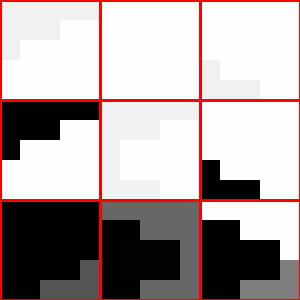
\includegraphics[width=0.2\linewidth]{triangle/som}\hfill
			
\includegraphics[width=0.2\linewidth]{triangle/triangle}
		\end{subfigureth}
		\caption[Compression et décompression d'image]{Schéma simplifié du processus de compression et de reconstruction d'une image, avec ici seulement 9 neurones et 25 imagettes.}\label{fig:img:comp_ex}
	\end{figureth}

	\subsection{La gestion des canaux (couleurs)}\label{sec:img:colors}

	Nous avons jusque là vu comment apprendre une image ayant une seule valeur par pixel (soit des images en nuances de gris). Cependant la majorité des dispositifs de capture actuels fournissent des images en couleur, c'est à dire trois canaux. Nous allons voir dans cette section comment transposer l'apprentissage, la compression et la reconstruction à des images à un nombre arbitraire de canaux par pixels.

	Une approche possible serait de séparer l'image par composante. Une image RVB par exemple donnerait trois images en niveau de gris, une R, une V et une B. Deux options s'offrent ensuite à nous. Soit utiliser une seule SOM pour apprendre toutes les images ainsi extraites en espérant que les différentes formes présentes dans chaque composante soient assez similaires entre elles. Cela augmente aussi les données que la SOM doit apprendre, car on vient de multiplier la taille de notre base d'apprentissage par le nombre de canaux. Ces données doivent être aussi cohérentes dans l'espace d'entrée pour que la réduction dimensionnelle se fasse correctement. Soit utiliser une SOM par composante pour apprendre chaque canal séparément, et de regrouper ensuite les différents canaux reconstitués en une image couleur. 
	
	Cependant ces deux approches ont un défaut majeur pour la compression d'images (ainsi que la détection de nouveauté par conséquent), c'est la création d'aberrations chromatiques dans l'image reconstituée. En effet, les canaux étant appris séparément avant d'être recombinés, la reconstruction peut donner pour certains pixels des teintes de couleurs qui n'existaient pas dans l'image de base, et très saillants visuellement. Par exemple un pixel blanc dans l'image d'entrée (avec une forte composante R, V et B), lorsque reconstitué par la SOM peut être bien reconstitué dans deux composantes (V et B par exemple), et mal reconstitué dans la troisième (R) avec une valeur beaucoup plus faible que dans l'image de base (cela arrive car notre calcul de distance minimise ). Par conséquent ce pixel aura une couleur turquoise dans l'image reconstituée à la place de blanc. Cette erreur minimise bien la distance avec l'image de base, et ce n'est que visuellement que les changements de teintes sont apparents et dégradent proportionnellement plus la qualité de l'image que que l'erreur mesurée.

	Une meilleure approche consiste à inclure tous les canaux directements dans les imagettes. Chaque imagette devient donc une imagette en couleur, et sa taille augmente donc en conséquence. Une imagette de 10 par 10 pixels par exemple qui donnerait un vecteur prototype de taille 100, passe à 300 avec les trois couleurs. L'apprentissage et la reconstruction se déroulent de la même manière que dans la SOM classique. Il faut aussi noter que l'ordre n'a pas d'importance dans les vecteurs prototypes, on peut arranger les valeurs en RGBRGBRGB tout comme RRRGGGBBB sans que cela ne change le résultat, le calcul de distance euclidienne étant indépendant de l'ordre des coordonnées.

	\begin{figureth}
		\begin{subfigureth}{0.48\textwidth}
			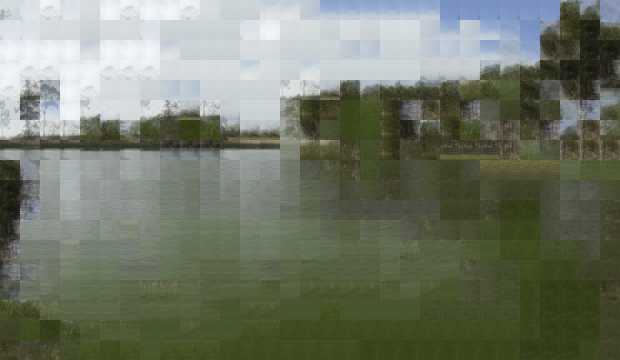
\includegraphics[width=\linewidth]{fusioned_color}\caption{Couleurs fusionnées}	
		\end{subfigureth}
		\begin{subfigureth}{0.48\textwidth}
			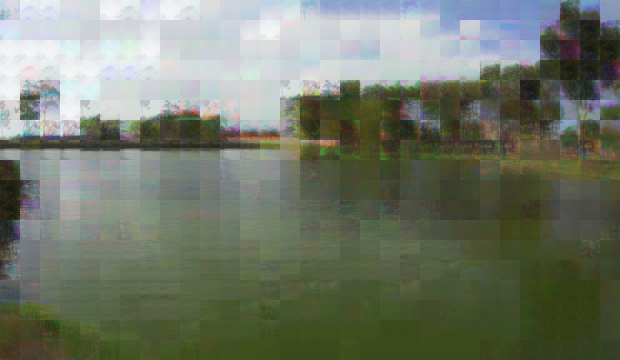
\includegraphics[width=\linewidth]{separated_colors}\caption{Couleurs séparées}	
		\end{subfigureth}
		\caption[Représentation d'une image]{Comparaison entre une image avec des couleurs fusionnées et la même image avec des couleurs séparées qui présente des artefacts visuels.[Faire un exemple plus visuel]}\label{fig:img:rep}
	\end{figureth}

	\newpage
	\section{Notre détection de nouveauté}

	Nous avons à partir des différentes propriétés de nos modèles neuronaux développé des processus de détection de nouveauté. Ces processus ne sont pas intrinsèques à nos modèles, c'est à dire que nos modèles neuronaux n'ont pas été définis dans le but d'effectuer une détection de nouveauté. Elle est une propriété émergente de ces modèles. Nous présentons ces deux méthodes dans cette section. La première est basée sur la propriété de quantification vectorielle et la seconde sur la topologie.

	\subsection{Détection avec quantification vectorielle}

	\begin{figureth}
		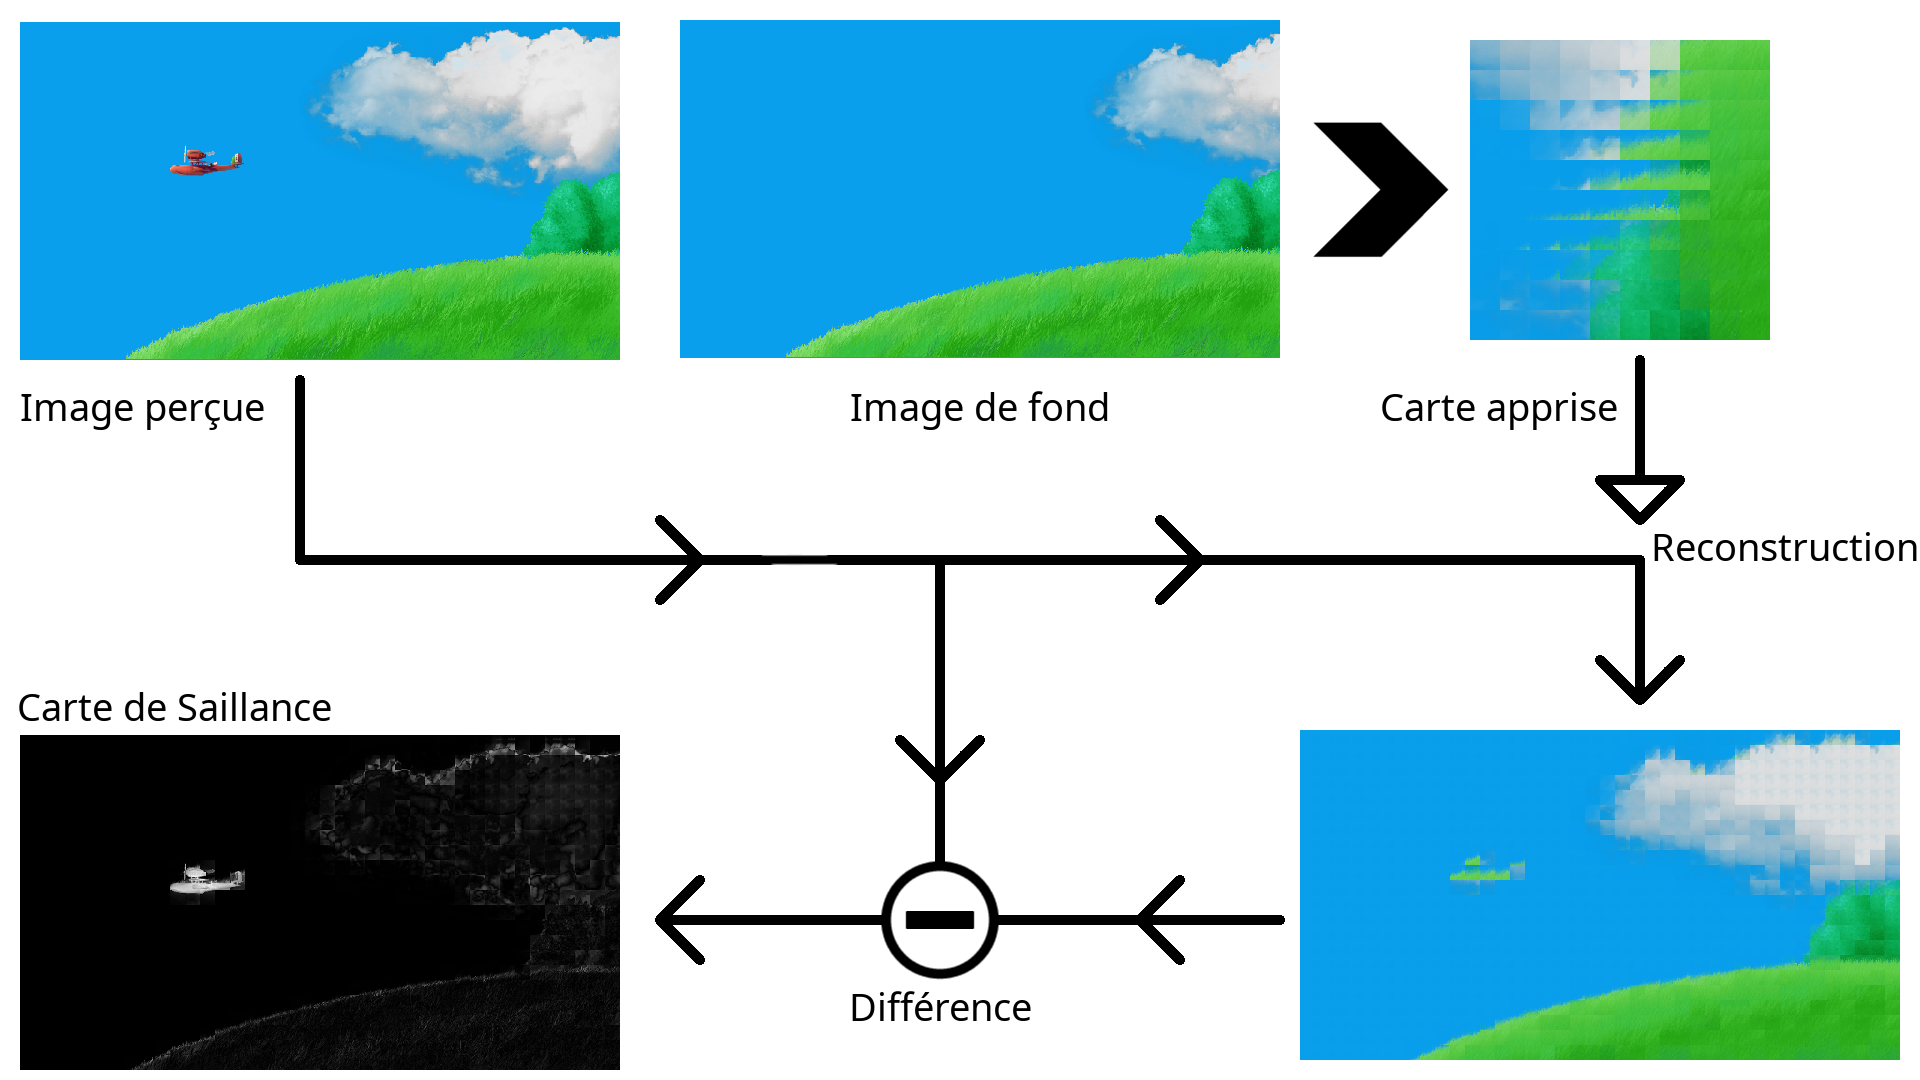
\includegraphics[width=\linewidth]{saliency_map_generation}
		\caption[Détection de nouveauté par quantification vectorielle]{On peut observer qu'il y a eu deux changements entre le fond et l'image perçue : un avion est apparu et les nuages ont bougé. Les nuages, déjà présents dans le fond sont bien reconstruits. L'avion cependant est nouveau, et n'est pas bien reconstruit. Ainsi la différence entre l'image perçue et la reconstruction rend plus saillant l'avion que les nuages. Contrairement à une simple différence entre le fond et l'image perçue, où les deux seraient saillants. Nous avons représenté le modèle appris comme étant une SOM sur cette figure, cependant il peut s'agir de n'importe quel modèle de quantification vectorielle.}\label{fig:img:vq}
	\end{figureth}

	La détection par quantification vectorielle repose sur l'erreur de reconstruction de la nouvelle image provenant du capteur. Cette erreur est la différence entre la nouvelle image et celle reconstruite avec le modèle de VQ ayant effectué son apprentissage sur l'image de fond.

	Il y a deux cas à considérer pour chaque imagette de la nouvelle image du capteur : soit la nouvelle imagette est similaire à une partie quelconque de l'arrière-plan appris, soit quelque chose de nouveau est présent dans l'imagette. Dans le premier cas, le neurone représentatif de cette imagette sera proche de celle-ci, c'est à dire que les poids du neurones et de l'imagette seront proches. L'erreur de reconstuction de cette imagette sera faible, surtout si la caméra est statique, mais avec une petite différence toujours présente en raison des pertes de la compression et des changements naturels de l'environnement visuel.
	
	Cependant, dans le second cas, le neurone représentatif de l'imagette sera éloigné de celle-ci, dans le sens où ses poids seront très différents de ceux de l'imagette. Car la nouveauté est par définition quelque chose qui n'était pas présent dans l'arrière-plan et donc quelque chose que le modèle n'a pas appris. Cela entraînera à une différence significative lors du calcul de la soustraction entre l'image perçue et sa reconstruction à l'endroit de la nouveauté. Ce processus est illustré dans la figure \ref{fig:img:vq}. 

	Ce processus a l'avantage d'être précis au niveau du pixel pour la mise en évidence des changements [Préciser que la taille des imagettes limites quand même la précision]. Il est aussi théoriquement insensible au déplacement d'objets du fond pour la détection de la nouveauté. Cependant, il peut être bruité en raison de l'apprentissage imparfait de la VQ et de la variabilité naturelle de l'environnement.

	\subsection{Détection avec distance neurale}

	\begin{figureth}
		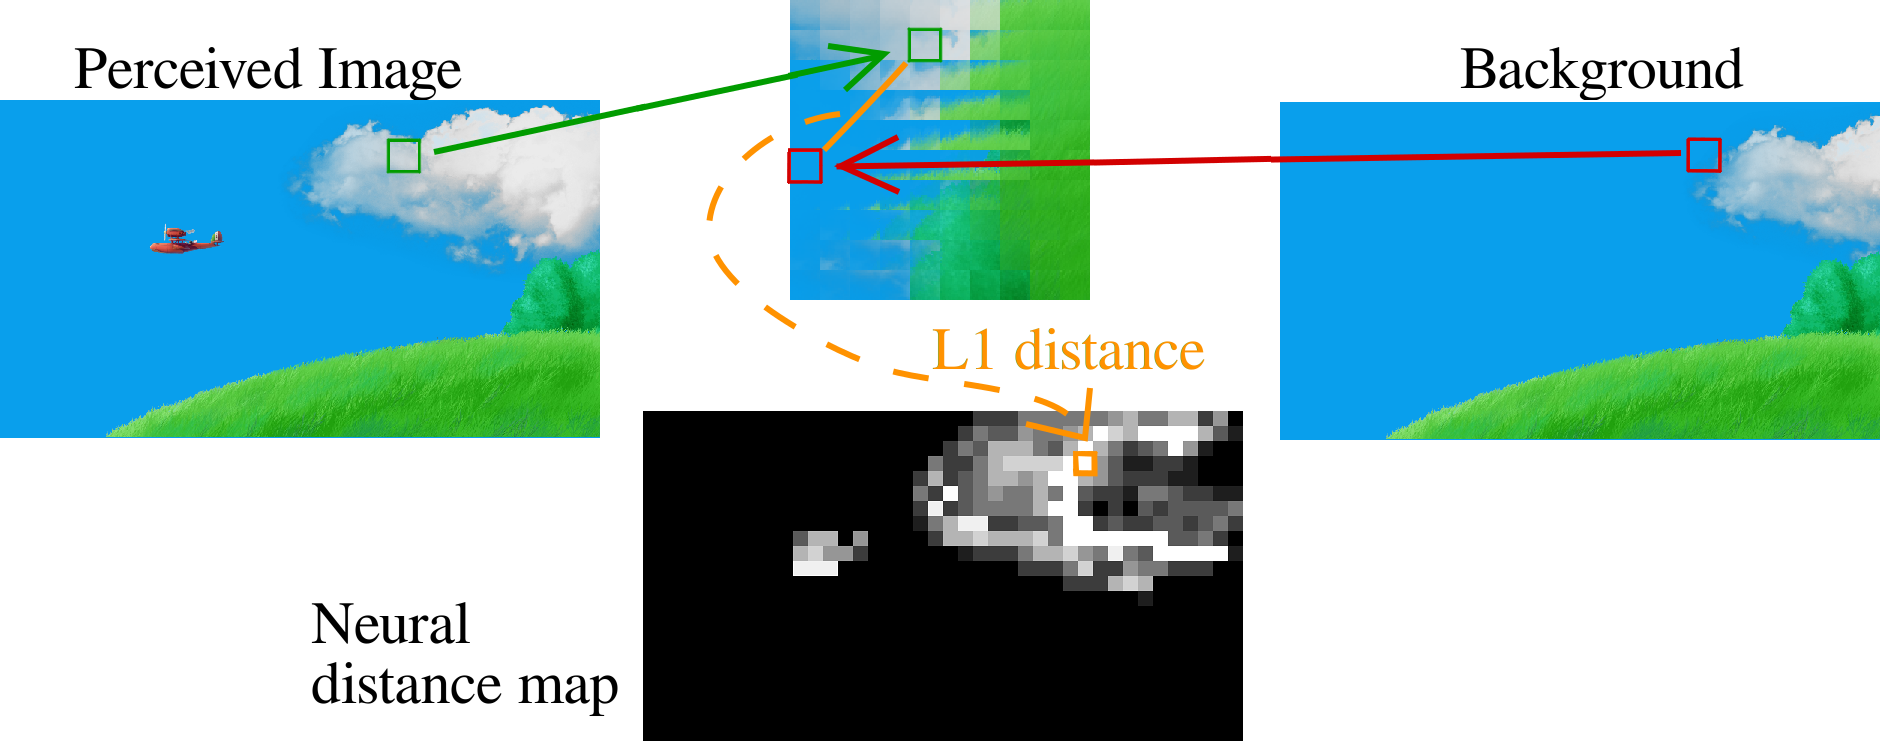
\includegraphics[width=\linewidth]{neural_distance_modulation_v2}
		\caption[Détection de nouveauté avec topologie]{Le processus présenté ici concerne une position dans l'image, et il est répété sur toute l'image pour obtenir la carte de distances neurales en bas. Nous avons représenté le modèle appris comme étant une SOM sur cette figure, cependant il peut s'agir de n'importe quel modèle avec une topologie regroupant les éléments proches.[Traduire la figure en français]}\label{fig:img:topo}
	\end{figureth}

	La détection avec distance neurale se base sur les propriétés topologiques du modèle pour trouver la nouveauté dans une image. La topologie est ce qui relie les différents neurones de modèle par leur proximité : les neurones proches dans la topologie ont appris des poids similaires.

	Après avoir effectué l'apprentissage du modèle, nous mémorisons la liste des positions dans la carte des neurones représentant trouvés pour toutes les imagettes.Lorsqu'une nouvelle image est présentée au capteur, nous effectuons le processus de reconstruction comme dans la première méthode de détection de la nouveauté. Nous nous intéressons uniquement à la liste des positions dans la carte des neurones représentant trouvés pour toutes les imagettes de la nouvelle image. En comparant les deux listes, nous pouvons trouver des changements dans les positions des BMU pour chaque emplacement d'imagette. Si la BMU est la même entre le fond et la nouvelle image à un endroit, alors il n'y a probablement pas de nouveauté à cet endroit. S'il y a une différence entre les deux BMU, alors il pourrait y avoir de la nouveauté à cet endroit. Pour quantifier cette différence, nous calculons la distance topologique qui les sépare sur la carte. La distance topologique est définie par le nombre de nœuds qui sont traversés par le chemin le plus court entre les deux BMU dans la topologie de la carte. Dans la SOM classique basée sur une grille, il s'agit simplement de la distance L1.

	Grâce à ces distances, nous pouvons créer une carte de saillance où des distances élevées dans la topologie signifient des changements significatifs dans l'image, car la proximité dans la topologie signifie la proximité dans l'espace d'entrée. Cette méthode permet d'obtenir une carte de saillance plus robuste, avec moins de bruit que la version avec la VQ. La précision est limitée à la taille des imagettes et il n'y a pas d'inhibition pour les éléments déjà connus qui se sont déplacés dans la fond. Le processus est illustré dans la figure \ref{fig:img:topo}.

	\subsection{Considérations pour la combinaison}
	
	Une fois les deux cartes de saillance générées, il est nécessaire de les combiner pour n'avoir qu'un seul résultat qui représentera la sortie de notre système. Il existe un très grand nombre de façons de le faire cette combinaison, et il existe dans la littérature des modèles qui se basent sur une bonne combinaison de différentes cartes de saillance pour obtenir de meilleurs résultats [citation]. Dans notre cas, nous avons avons préféré utiliser une combinaison simple de nos deux cartes de saillance. C'est à dire qu'elle n'utilise pas de paramètres, pour ne pas ajouter une variable de plus à optimiser. Nous souhaitons aussi bénéficier de la complémentarité des deux cartes de saillances. La solution la plus simple est de multiplier les deux cartes ensemble. Ainsi, sera considéré comme nouveauté dans la carte de sortie, ce qui apparaît comme nouveauté en même temps dans les deux cartes de saillance. Car $\textit{petit} \times \textit{petit} = \textit{petit}$, $\textit{grand} \times \textit{petit} = \textit{petit}$ et seulement $\textit{grand} \times \textit{grand} = \textit{grand}$. Le bruit présent dans la carte résultant de la quantification vectorielle et qui n'est pas présent dans la carte topologique disparaît de la carte finale. Il en va de même pour les mouvements qui ne sont pas des nouveautés qui apparaissent dans la carte topologique, mais pas dans la carte de quantification vectorielle.

	Un problème qui peut apparaître avec cette méthode est la trop petite valeur du résultat et le déséquilibre d'impact de nos deux cartes, car nos cartes de saillance sont toutes les deux définies entre 0 et 1. Il est possible que des situations arrivent lors desquelles les deux cartes ont un impact disproportionnel sur le résultat. Par exemple si la saillance a une valeur de 0.2 sur une carte et 0.8 sur l'autre, alors la seconde aura plus d'impact sur les valeurs de la sortie finale. De même, en multipliant deux nombres compris entre 0 et 1, le résultat sera forcément inférieur à chacun des deux nombres. Cela a un effet réducteur sur toutes les valeurs de la carte de saillance finale. La solution que nous avons choisi à ces deux problèmes, est de re-normaliser les deux cartes de saillances avant de les multiplier. C'est à dire que l'on rééchelonne l'ensemble de la carte en mettant la valeur maximum de la carte à 1 et le minimum à 0 et d'étaler les valeurs intermédiaires entre les deux pour conserver le même espacement relatif entre elles. Cela a pour effet d'éviter une trop grande disproportion d'impact entre les deux cartes sans résoudre complètement le problème cependant. Car on re-normalise avec le maximum, et non avec la possible valeur de la nouveauté detectée. Cela permet également d'avoir un résultat avec des valeurs généralement plus hautes. Cependant, cela vient aussi avec des désavantages, comme par exemple le fait que si il n'y a pas de signal dans l'entrée, le maximum des cartes de saillance sera quand même 1. On pourrait observer des signaux positifs dans la sortie alors que l'entrée et les cartes de saillances n'en montrent pas. En pratique, cela est peu fréquent car la valeur maximum dans un cas où il n'y a pas de signal en entrée vient du bruit, et est donc décorellée entre les deux cartes, et disparaîtra lors de la multiplication. De plus, la taille du signal d'entrée compte, et il est peu probable que du bruit seul puisse créer une zone de signal assez large pour être confondu avec une vraie nouveauté.

	\newpage
	\section{Protocole expérimental}

	Cette section regroupe l'ensemble des considérations pratiques pour la réalisation de nos expériences. Nous présenterons la base de donnée utilisée, comment ces données ont été préparées, les différentes métriques que nous avons mesuré et les paramétrages de nos modèles.

	\subsection{Présentation de la base de données}

	Il n'existe pas à notre connaissance de base de données de détection de nouveauté respectant nos hypothèses de caméra statique, de [...]. Une alternative se trouve dans la base de donnée CDnet \cite{wang-cdnet}. Elle a pour objectif d'uniformiser les résultats dans un domaine proche de la détection de nouveauté ; la détection de changement. Les deux domaines peuvent sembler similaires au premier abord car les deux approches visent la même application réelle. Cependant cela cache une différence conceptuelle. La détection de changement se concentre sur le mouvement pour séparer le fond des objets intéressants dans une image. La détection de nouveauté quand à elle se réfère à une représentation apprise de l'environnement (discuté plus en détail dans la section [...]). Dans les captures vidéos réelles, les deux sont généralement équivalents dû au fait que lorsqu'une nouveauté apparaît, elle le fait généralement en se déplaçant. En pratique cela veut dire que la majorité de CDnet peut être utilisé pour de la détection de nouveauté. Nous présenterons les catégories et vidéos que l'ont a utilisé, et des exemples de vidéos qui n'ont pas été retenues avec des explications dans la suite.
	
	CDnet regroupe 53 séquences vidéos originaires de sources variées. Elles proviennent principalement de caméras de surveillance ou de captures effectuées par des chercheurs pour leur propres besoins. Il n'y a que des captures réelles, sans images synthétiques de scènes intérieures et extérieures. Les vidéos sont toutes en couleur, sauf pour deux catégories \textit{thermal} et \textit{turbulences}, et de résolution assez faible, allant de $320 \times 240$ de $720 \times 486$ pixels. Elles sont groupées en 11 catégories de 4 à 6 vidéos sensées représenter une variété de difficultés que peuvent rencontrer les modèles de détection de changement. Il existe cependant un certain biais dans CDnet, car il est fortement orienté vers de la détection de personnes et de véhicules. Ces catégories sont présentées dans les figures suivantes.

	Parmi les 11 catégories de CDnet, nous avons décidé d'en utiliser 8 complètement, d'utiliser une version réduite pour 2 d'entre elles et d'en enlever une. Les deux catégories réduites sont \textit{Intermittent Object Motion} et \textit{Low framerate}. La réduction consiste à enlever une partie des vidéos qui ne correspondaient pas à notre tâche de ces catégories et de conserver les autres. Une illustration de la différence entre la détection de changements et la détection de nouveauté qui est la source de la suppression est montré sur la figure \ref{fig:cdnet:diff}. La catégorie que nous avons décidé de ne pas du tout utiliser car elle ne correspondait pas à notre scénario est \textit{Pan tilt zoom}. C'est une catégorie un peu spéciale car elle change une partie fondamentale du scénario. La caméra n'est plus statique mais effectue des roations et des zooms ce qui change significativement son environnement visuel.


	\begin{figureth}
		\begin{subfigureth}{0.24\textwidth}
			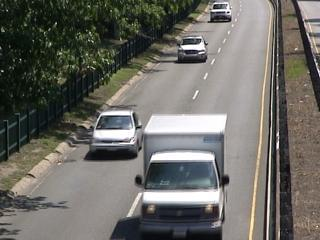
\includegraphics[width=\linewidth]{CDNET/baseline/in000277}\caption{Highway}	
		\end{subfigureth}
		\begin{subfigureth}{0.24\textwidth}
			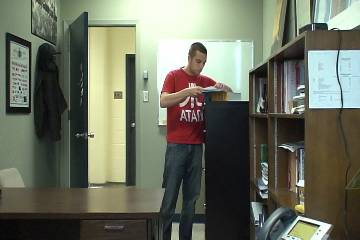
\includegraphics[width=\linewidth]{CDNET/baseline/in000895}\caption{Office}	
		\end{subfigureth}
		\begin{subfigureth}{0.24\textwidth}
			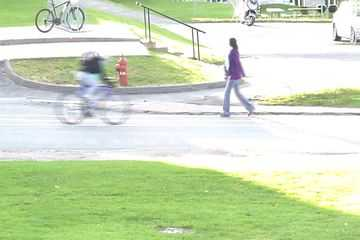
\includegraphics[width=\linewidth]{CDNET/baseline/in000473}\caption{Pedestrians}	
		\end{subfigureth}
		\begin{subfigureth}{0.24\textwidth}
			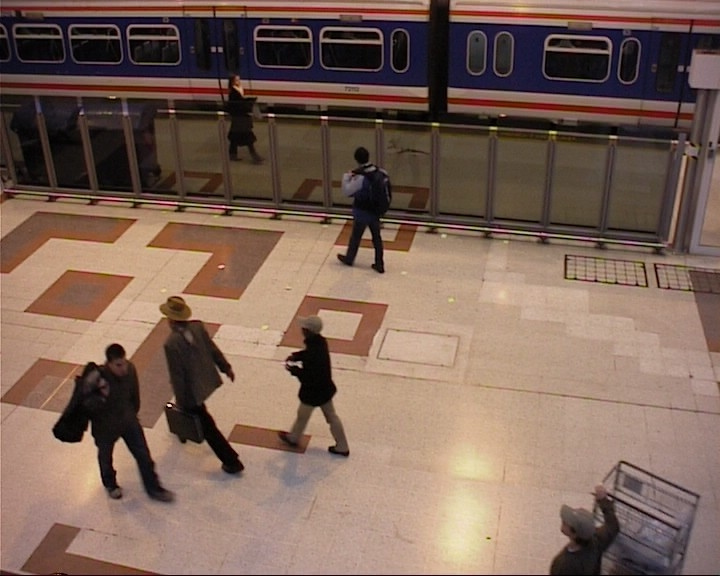
\includegraphics[width=\linewidth]{CDNET/baseline/in000118}\caption{PETS2006}	
		\end{subfigureth}
		\caption[Catégorie Baseline]{\textit{Baseline} : La catégorie de base qui comprend des scénarios typiques de détection de changement (traffic, piétons) sans difficultés particulières.}\label{fig:cdnet:baseline}
	\end{figureth}

	\begin{figureth}
		\begin{subfigureth}{0.24\textwidth}
			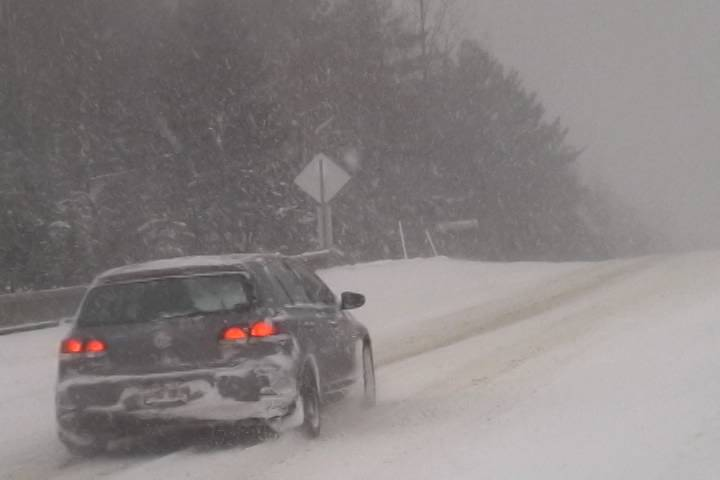
\includegraphics[width=\linewidth]{CDNET/badWeather/in000810}\caption{Snowfall}	
		\end{subfigureth}
		\begin{subfigureth}{0.24\textwidth}
			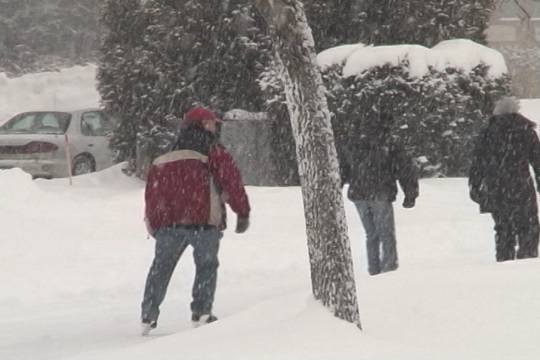
\includegraphics[width=\linewidth]{CDNET/badWeather/in001951}\caption{Skating}	
		\end{subfigureth}
		\begin{subfigureth}{0.24\textwidth}
			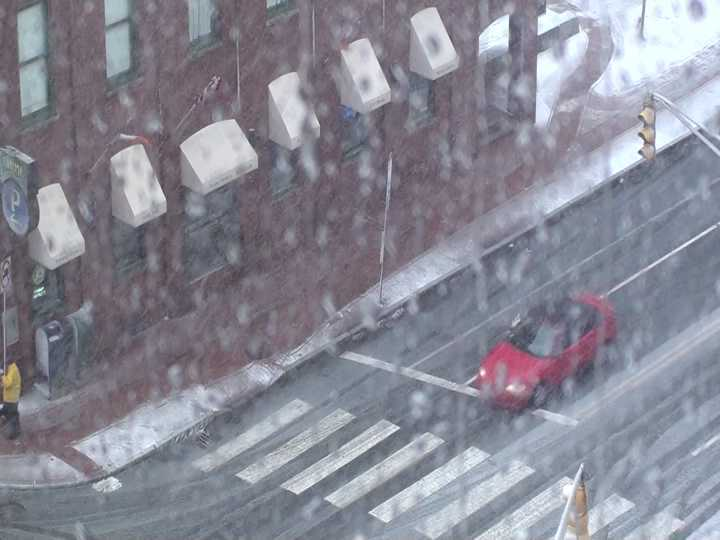
\includegraphics[width=\linewidth]{CDNET/badWeather/in002841}\caption{WetSnow}	
		\end{subfigureth}
		\begin{subfigureth}{0.24\textwidth}
			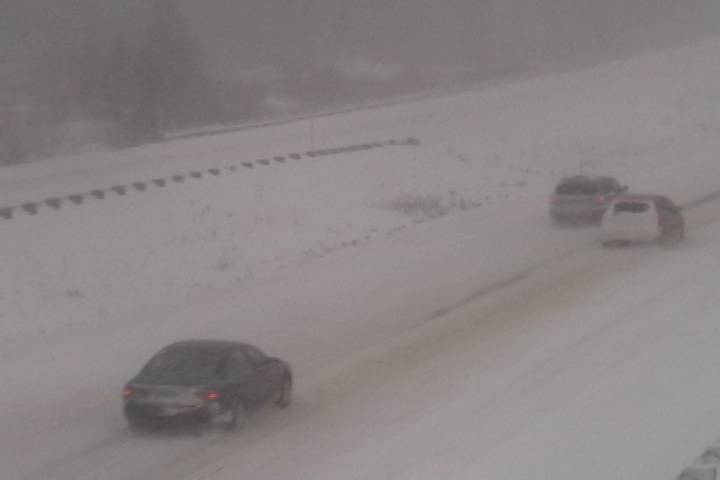
\includegraphics[width=\linewidth]{CDNET/badWeather/in004863}\caption{Blizzard}	
		\end{subfigureth}
		\caption[Catégorie Bad weather]{\textit{Bad weather} : Cette catégorie comprend des variations du scénario de base avec une météo dégradée. La difficulté principale vient de la neige qui tombe, et du changment de l'environnement avec les traces de pneus sur la neige par exemple.}\label{fig:cdnet:badweather}
	\end{figureth}

	\begin{figureth}
		\begin{subfigureth}{0.24\textwidth}
			\includegraphics[width=\linewidth]{CDNET/cameraJitter/in000145}\caption{Sidewalk}	
		\end{subfigureth}
		\begin{subfigureth}{0.24\textwidth}
			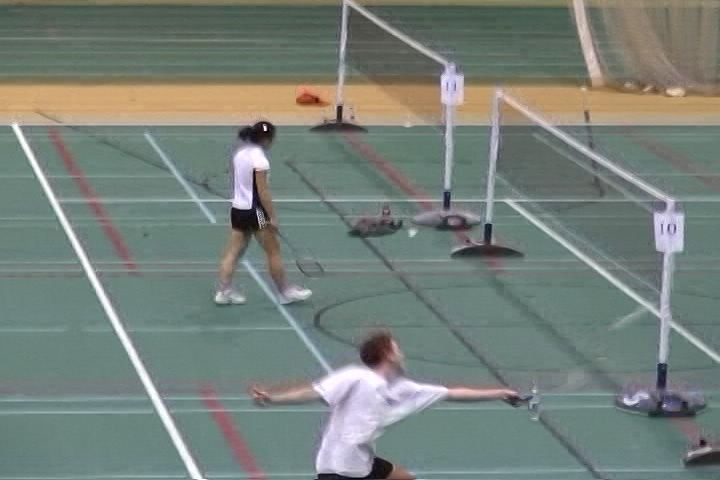
\includegraphics[width=\linewidth]{CDNET/cameraJitter/in000187}\caption{Badminton}	
		\end{subfigureth}
		\begin{subfigureth}{0.24\textwidth}
			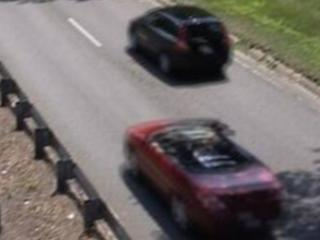
\includegraphics[width=\linewidth]{CDNET/cameraJitter/in000355}\caption{Traffic}	
		\end{subfigureth}
		\begin{subfigureth}{0.24\textwidth}
			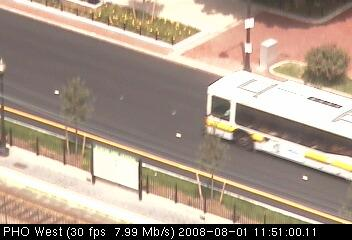
\includegraphics[width=\linewidth]{CDNET/cameraJitter/in002287}\caption{Boulevard}	
		\end{subfigureth}
		\caption[categorie camera jitter]{\textit{Camera Jitter} : Ces vidéos proviennent de caméras instables à cause de vent fort ou d'autres raisons. Elles ont de façon irrégulière des translations verticales et horizontales  rapides et de petite amplitude.}\label{fig:cdnet:jitter}
	\end{figureth}

	\begin{figureth}
		\begin{subfigureth}{0.24\textwidth}
			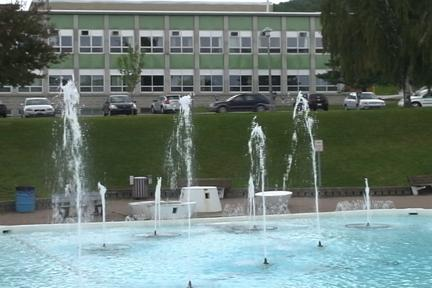
\includegraphics[width=\linewidth]{CDNET/dynamicBackground/in000716}\caption{Fountain01}	
		\end{subfigureth}
		\begin{subfigureth}{0.24\textwidth}
			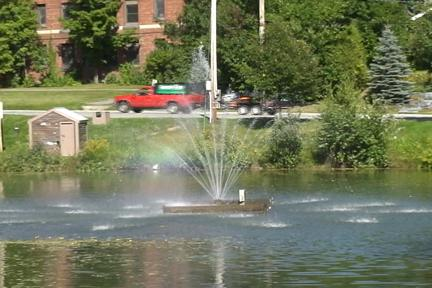
\includegraphics[width=\linewidth]{CDNET/dynamicBackground/in000720}\caption{Fountain02}	
		\end{subfigureth}
		\begin{subfigureth}{0.24\textwidth}
			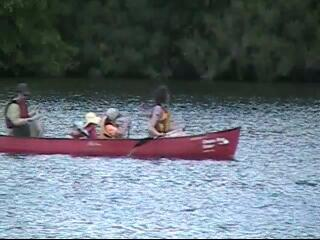
\includegraphics[width=\linewidth]{CDNET/dynamicBackground/in000937}\caption{Canoe}	
		\end{subfigureth}\\
		\begin{subfigureth}{0.24\textwidth}
			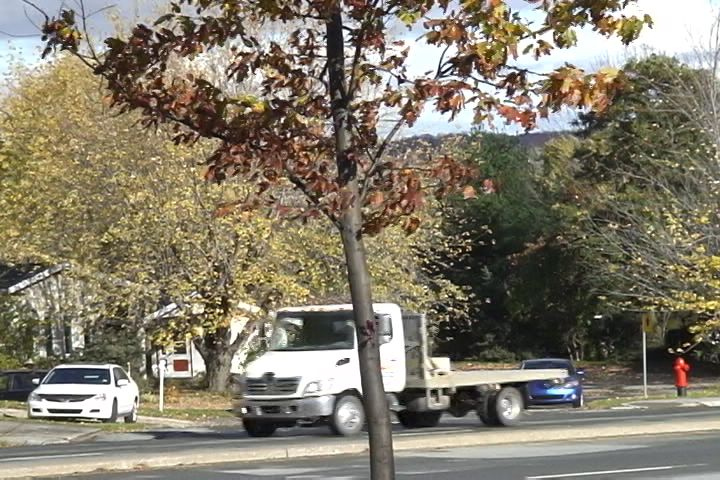
\includegraphics[width=\linewidth]{CDNET/dynamicBackground/in001504}\caption{Fall}	
		\end{subfigureth}
		\begin{subfigureth}{0.24\textwidth}
			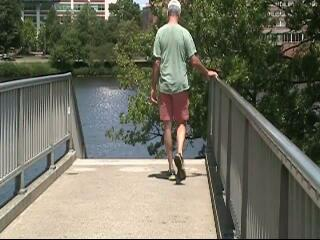
\includegraphics[width=\linewidth]{CDNET/dynamicBackground/in002519}\caption{Overpass}	
		\end{subfigureth}
		\begin{subfigureth}{0.24\textwidth}
			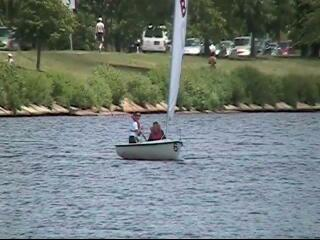
\includegraphics[width=\linewidth]{CDNET/dynamicBackground/in007726}\caption{Boats}	
		\end{subfigureth}
		\caption[Categorie Dynamic Background]{\textit{Dynamic Background} : La difficulté se porte sur le contenu du fond qui est changeant. Il peut s'agir d'eau ou d'arbres qui bougent dans le vent.}\label{fig:cdnet:dynamic}
	\end{figureth}

	\begin{figureth}
		\begin{subfigureth}{0.24\textwidth}
			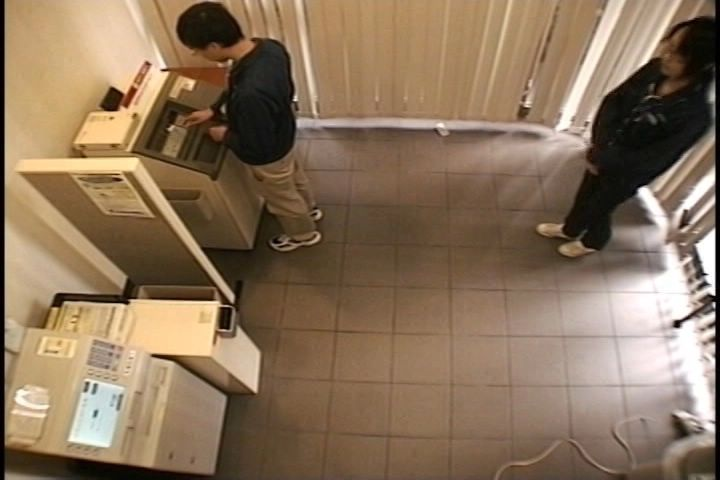
\includegraphics[width=\linewidth]{CDNET/shadow/in000260}\caption{CopyMachine}
		\end{subfigureth}
		\begin{subfigureth}{0.24\textwidth}
			\includegraphics[width=\linewidth]{CDNET/shadow/in000320}\caption{PeopleInShade}
		\end{subfigureth}
		\begin{subfigureth}{0.24\textwidth}
			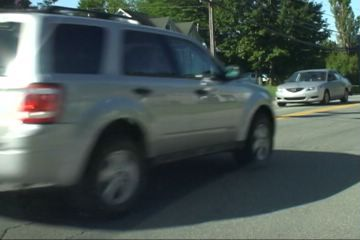
\includegraphics[width=\linewidth]{CDNET/shadow/in000358}\caption{Bungalows}	
		\end{subfigureth}\\
		\begin{subfigureth}{0.24\textwidth}
			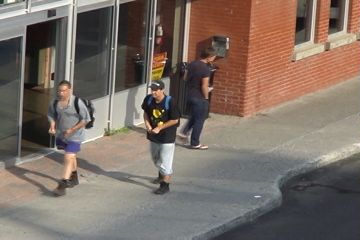
\includegraphics[width=\linewidth]{CDNET/shadow/in001015}\caption{BusStation}	
		\end{subfigureth}
		\begin{subfigureth}{0.24\textwidth}
			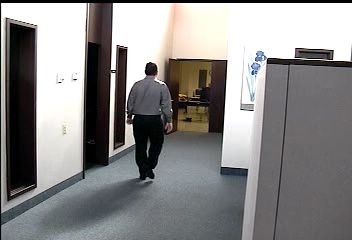
\includegraphics[width=\linewidth]{CDNET/shadow/in001210}\caption{Cubicle}
		\end{subfigureth}
		\begin{subfigureth}{0.24\textwidth}
			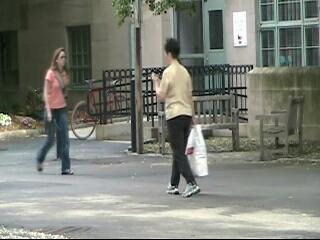
\includegraphics[width=\linewidth]{CDNET/shadow/in001850}\caption{Backdoor}	
		\end{subfigureth}
		\caption[Categorie Shadow]{\textit{Shadow} : Catégorie de vidéos qui présente plus d'ombres que la moyenne.}\label{fig:cdnet:shadow}
	\end{figureth}

	\begin{figureth}
		\begin{subfigureth}{0.24\textwidth}
			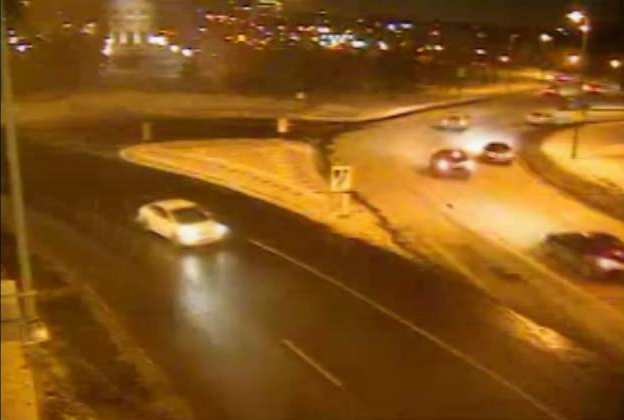
\includegraphics[width=\linewidth]{CDNET/nightVideos/in000060}\caption{WinterStreet}	
		\end{subfigureth}
		\begin{subfigureth}{0.24\textwidth}
			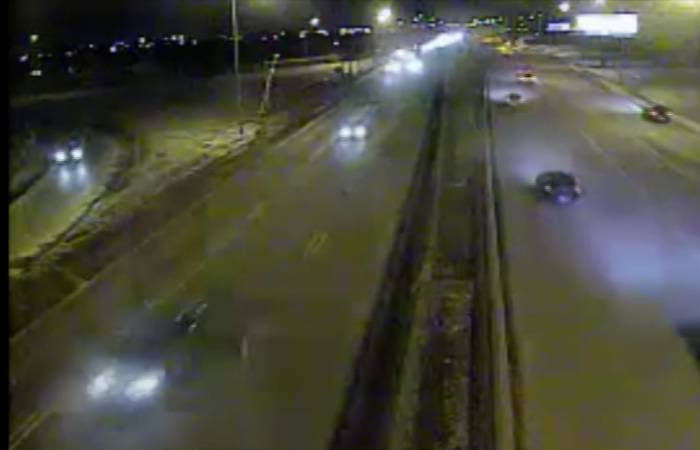
\includegraphics[width=\linewidth]{CDNET/nightVideos/in000125}\caption{FluidHighway}	
		\end{subfigureth}
		\begin{subfigureth}{0.24\textwidth}
			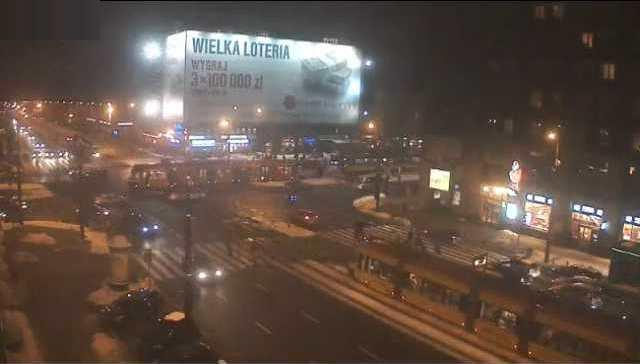
\includegraphics[width=\linewidth]{CDNET/nightVideos/in000150}\caption{BusyBoulevard}	
		\end{subfigureth}\\
		\begin{subfigureth}{0.24\textwidth}
			\includegraphics[width=\linewidth]{CDNET/nightVideos/in000320}\caption{TramStation}	
		\end{subfigureth}
		\begin{subfigureth}{0.24\textwidth}
			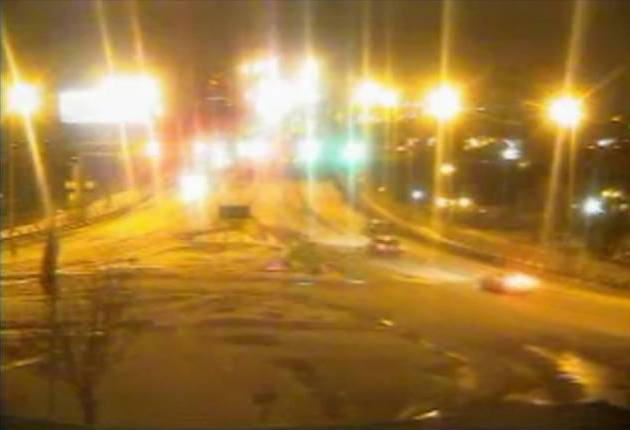
\includegraphics[width=\linewidth]{CDNET/nightVideos/in000362}\caption{BridgeEntry}	
		\end{subfigureth}
		\begin{subfigureth}{0.24\textwidth}
			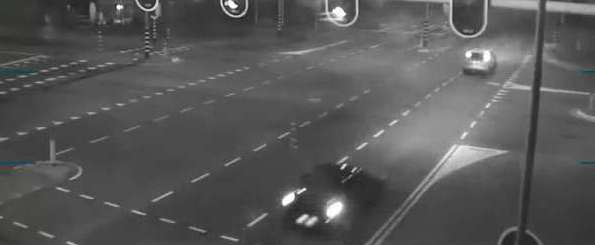
\includegraphics[width=\linewidth]{CDNET/nightVideos/in000671}\caption{StreetCornerAtNight}	
		\end{subfigureth}
		\caption[Categorie Night Videos]{\textit{Night Videos} : Vidéos de nuit avec un contraste fort entre l'obscurité ambiante et les lumières artificielles de l'éclairage public et des phares de voitures.}\label{fig:cdnet:night}
	\end{figureth}

	\begin{figureth}
		\begin{subfigureth}{0.24\textwidth}
			\includegraphics[width=\linewidth]{CDNET/thermal/in000145}\caption{Park}
		\end{subfigureth}
		\begin{subfigureth}{0.24\textwidth}
			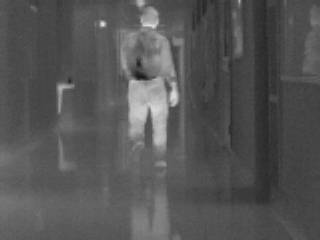
\includegraphics[width=\linewidth]{CDNET/thermal/in000800}\caption{Corridor}	
		\end{subfigureth}
		\begin{subfigureth}{0.24\textwidth}
			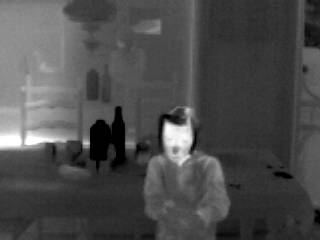
\includegraphics[width=\linewidth]{CDNET/thermal/in000840}\caption{DiningRoom}	
		\end{subfigureth}\\
		\begin{subfigureth}{0.24\textwidth}
			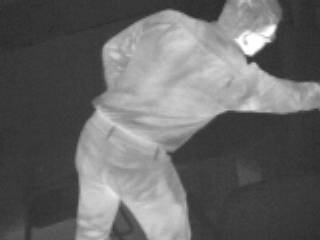
\includegraphics[width=\linewidth]{CDNET/thermal/in001050}\caption{Library}	
		\end{subfigureth}
		\begin{subfigureth}{0.24\textwidth}
			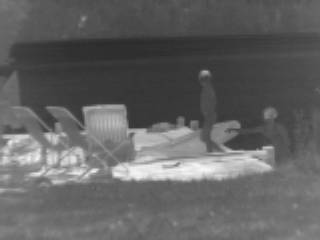
\includegraphics[width=\linewidth]{CDNET/thermal/in002220}\caption{LakeSide}	
		\end{subfigureth}
		\caption[Categorie thermal]{\textit{Thermal} : Ces vidéos ont été prises par une caméra infrarouge et sont en niveau de gris.}\label{fig:cdnet:shadow}
	\end{figureth}

	\begin{figureth}
		\begin{subfigureth}{0.24\textwidth}
			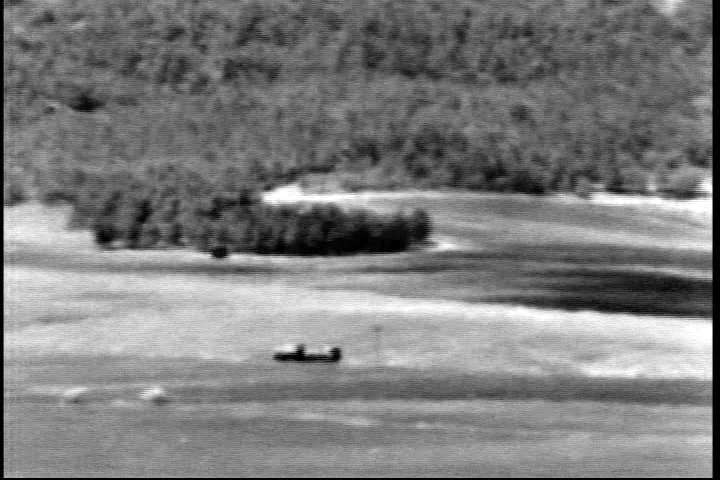
\includegraphics[width=\linewidth]{CDNET/turbulence/in000425}\caption{Turbulence0}	
		\end{subfigureth}
		\begin{subfigureth}{0.24\textwidth}
			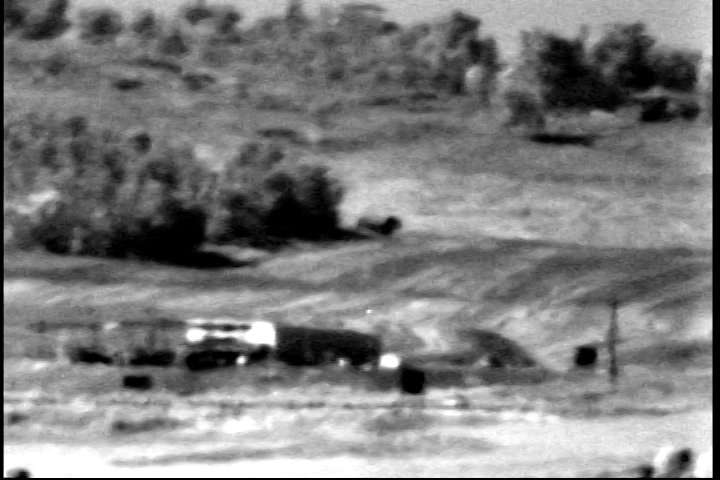
\includegraphics[width=\linewidth]{CDNET/turbulence/in000920}\caption{Turbulence1}	
		\end{subfigureth}
		\begin{subfigureth}{0.24\textwidth}
			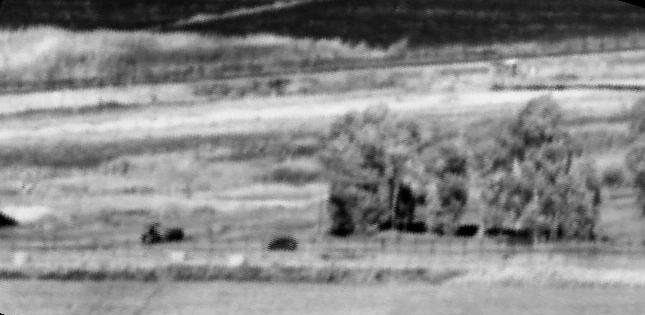
\includegraphics[width=\linewidth]{CDNET/turbulence/in000140}\caption{Turbulence2}	
		\end{subfigureth}
		\begin{subfigureth}{0.24\textwidth}
			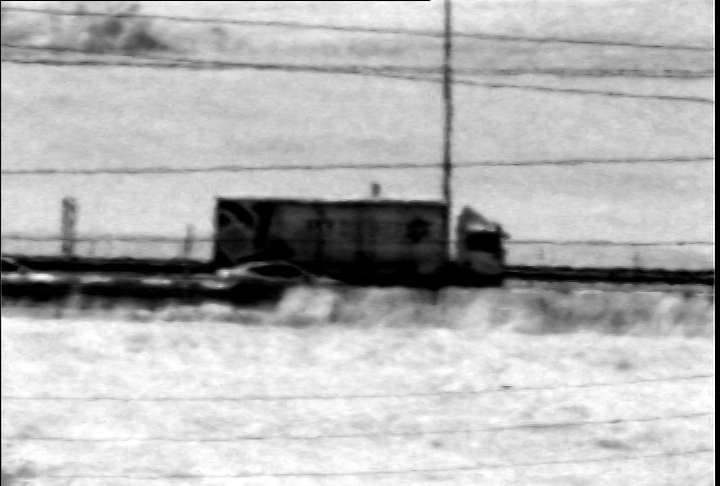
\includegraphics[width=\linewidth]{CDNET/turbulence/in000195}\caption{Turbulence3}	
		\end{subfigureth}
		\caption[Categorie turbulence]{\textit{Turbulence} : Catégorie qui regroupe des vidéos provenant d'une même caméra infrarouge. Les captures ont été faites avec un objectif longue distance filmant des scènes à 5 à 15 km de l'objectif. Elle présente de nombreuses distortions et turbulences atmosphérique dûs à la chaleur et à la distance.}\label{fig:cdnet:turbulence}
	\end{figureth}
	
	\begin{figureth}
		\begin{subfigureth}{0.24\textwidth}
			\includegraphics[width=\linewidth]{CDNET/intermittentObjectMotion/in001000}\caption{StreetLight}
		\end{subfigureth}
		\begin{subfigureth}{0.24\textwidth}
			\includegraphics[width=\linewidth]{CDNET/intermittentObjectMotion/in001300}\caption{Sofa}	
		\end{subfigureth}
		\begin{subfigureth}{0.24\textwidth}
			\includegraphics[width=\linewidth]{CDNET/intermittentObjectMotion/in001350}\caption{Tramstop}	
		\end{subfigureth}
		\caption[Categorie intermittent object motion - Reduced]{\textit{Intermittent object motion Reduced} : Cette catégorie comprend des scénarios particuliers dans lesquels le changement est intermittent (c'est à dire qu'un objet passe de mouvement à statique ou inversement). Dans cette catégorie trois vidéos sur six on été conservées.}\label{fig:cdnet:shadow}
	\end{figureth}

	\begin{figureth}
		\begin{subfigureth}{0.24\textwidth}
			\includegraphics[width=\linewidth]{CDNET/lowFramerate/in000062}\caption{Turnpike}	
		\end{subfigureth}
		\begin{subfigureth}{0.24\textwidth}
			\includegraphics[width=\linewidth]{CDNET/lowFramerate/in000088}\caption{TramCrossroad}	
		\end{subfigureth}
		\begin{subfigureth}{0.24\textwidth}
			\includegraphics[width=\linewidth]{CDNET/lowFramerate/in000235}\caption{Tunnel Exit}	
		\end{subfigureth}
		\caption[Categorie low framerate - Reduced]{\textit{Low Framerate Reduced} : Cette catégorie regroupe des vidéos avec beaucoup de temps entre les images (entre 1 seconde et 6 secondes entre chaque image). Cela a pour but de pénaliser les approches à partir de flow optique, cependant notre approche n'est pas concernée. Trois vidéos sur les quatre ont été conservées. Seule une vidéo d'une marina a été retirée car la nouveauté (des bateaux) était trop similaire au fond, qui consiste en un grand nombre de bateaux ammarés.}\label{fig:cdnet:fps}
	\end{figureth}

	\begin{figureth}
		\begin{subfigureth}{0.24\textwidth}
			\includegraphics[width=\linewidth]{intermittentObjectExample/in001285}\caption{Voiture statique}	
		\end{subfigureth}
		\begin{subfigureth}{0.24\textwidth}
			\includegraphics[width=\linewidth]{intermittentObjectExample/gt001285}\caption{Vérité terrain}
		\end{subfigureth}
		\begin{subfigureth}{0.24\textwidth}
			\includegraphics[width=\linewidth]{intermittentObjectExample/in001815}\caption{Voiture en mouvement}	
		\end{subfigureth}
		\begin{subfigureth}{0.24\textwidth}
			\includegraphics[width=\linewidth]{intermittentObjectExample/gt001815}\caption{Vérité terrain}	
		\end{subfigureth}
		\caption[Difference entre nouveauté and changement]{Ces images sont extraites d'une vidéo de la catégorie \textit{Intermittent Object Motion} et illustrent la différence entre détection de changement et détection de nouveauté. Pour le changement la voiture fait partie du fond pendant une partie de la vidéo car elle est statique. Elle devient objet à détecter à partir du moment où elle commence à se déplacer. Pour la nouveauté, une telle distinction n'est pas possible. Soit elle fait partie du fond, et dans ce cas, même en mouvement elle ne devrait pas être considérée comme nouveauté. Soit elle ne fait pas partie du fond, et dans ce cas elle sera tout le temps considérée comme nouveauté, même lors de la séquence statique.}\label{fig:cdnet:diff}
	\end{figureth}

	\subsection{Métriques utilisées}

	Nous présenterons dans cette section les différentes métriques que l'on a utilisé pour évaluer nos modèles. Elles peuvent être regroupées en deux grandes catégories, la première est proche des modèles évalués (la SOM et les GNG), et essaye de mesurer la qualité d'apprentissage de ceux-ci. La seconde est plus orienté vers la tâche de détection de nouveauté. Cette deuxième catégorie utilise des métriques définies par CDnet pour comparer les résultats avec d'autres modèles. Celles-ci étant en grand nombre, nous nous sommes limités aux trois plus pertinentes qui sont la précision, le rappel et la f-measure.

	\subsubsection{MQE : Erreur de Quantification Moyenne}

	L'erreur de quantification moyenne (Mean Quantization Error) mesure la qualité de l'apprentissage ou de la reconstruction d'un algorithme de quantification vectorielle. C'est la somme des différences entre tous les vecteurs et leurs représentants, divisée par la dimension et le nombre de vecteurs pour obtenir l'erreur moyenne des composantes.
	
	\begin{equation}
		\text{MQE} = \frac{1}{dn} \sum_{i=0}^{n-1} |v_i - u_i|
	\end{equation}
	[glossaire pour la terminologie mathématique employée]

	Il s'agit d'une mesure simple à calculer et à comprendre. Elle présente néanmoins une mauvaise pondération des différences en pénalisant de la même manière les outliers que des différences diffuses. Par exemple un pixel qui aura un changement maximal (qui passe de noir à blanc par exemple) aura le même impact sur l'erreur que cent pixels qui passent de 0 à 0,01. Pour des images, le premier changement sera visible pour notre oeil, mais pas le second. Nous avons quand même choisi d'utiliser cette mesure dans nos expériences car elle représente le mieux la différence numérique des vecteurs à leurs représentants avant notre interprétation subjective de ces valeurs en images.

	\subsubsection{PSNR : Peak Signal to Noise Ratio}

	Le PSNR est une mesure très présente dans le domaine de la compression d'images \cite{huynh-psnr, korhonen-psnr}. Elle est similaire à la MQE, à la différence qu'il y a un carré à la place de la valeur absolue. D'où le nom de Mean Squared Quantization Error (MSQE) à calculer pour pouvoir obtenir le PSNR.
	
	\begin{equation}
		\text{MSQE} = \frac{1}{dn} \sum_{i=0}^{n-1} (v_i - u_i)^2
	\end{equation}
	\begin{equation}
		\text{PSNR} = 10 \log_{10} (\frac{1}{\text{MSQE}})
	\end{equation}

	Le PSNR est inspiré du domaine du traitement du signal, d'où la terminologie étrange pour de la compression d'image. L'idée est de trouver le ratio de bruit introduit par les pertes de la compression (Noise), avec l'intensité maximale du signal (Peak Signal), qui est la valeur maximum d'un pixel (1 dans notre cas). On peut noter que le PSNR fait passer d'un objectif de minimisation à une maximisation. L'ordre des valeurs reste inchangé et le logarithme ajoute un effet de rendement décroissant. Si on a par exemple trois valeurs de MSQE $x_1$, $y_1$ et $z_1$ avec $x_1 < y_1 < z_1$. $x_1$ sera la meilleure (la plus petite) et $z_1$ la moins bonne (la plus grande). Une fois converties en PSNR, les valeurs seront dans l'ordre suivant : $x_2 > y_2 > z_2$, avec $x_2$ étant toujours la meilleure et $z_2$ toujours la moins bonne, mais pour les raisons inverses cette fois : plus un PSNR est grand, mieux c'est. Un autre changement sera que si les intervalles étaient les même entre les trois valeurs, c'est à dire si $y_1 - x_1 = z_1 - y_1$ alors on aura $y_2 - x_2 < z_2 - y_2$, car le logarithme met plus d'espace deux hautes valeurs de MSQE qu'entre deux petites.

	Nous avons choisi d'utiliser le PSNR à la place de la MSQE car il est beaucoup plus facilement interprétable par des humain. Sa valeur typique étant comprise entre 0 et 100. L'utilisation du carré dans la MSQE entraine une plus grande pénalisation des outliers en comparaison à MQE. Ce n'est quand même pas une mesure objective de la qualité d'une image, car elle ne prend pas en compte certains paramètres comme le voisinage par exemple, qui sont importants dans notre perception humaine [réf biblio]. Puisque l'on utilise la distance quadratique dans nos algorithmes de quantification vectorielle, le PSNR est une métrique intéressante car elle est la valeur que notre algorithme tente de minimiser.
	
	\subsubsection{Précision}

	La précision mesure la proportion de pixels correctement labellisés en tant que nouveauté parmi tous les pixels que le modèle a labellisé comme nouveauté. La précision est comprise entre 0 et 1 et s'exprime souvent en pourcentage.
	
	\begin{equation}
		\text{Précision} = \frac{\text{Vrais Positifs}}{\text{Vrais Positifs} + \text{Faux Positifs}}
	\end{equation}

	\subsubsection{Rappel}

	Le rappel mesure la proportion de pixels correctement labellisés en tant que nouveauté parmi tous les pixels avec de la nouveauté dans la vérité terrain. Le rappel est compris entre 0 et 1 et s'exprime souvent en pourcentage.

	\begin{equation}
		\text{Rappel} = \frac{\text{Vrais Positifs}}{\text{Vrais Positifs} + \text{Faux Négatifs}}
	\end{equation}

	\subsubsection{F-measure}

	La précision et le rappel sont deux mesures qui, prises séparément, peuvent être facilement maximisées. Pour avoir une très bonne précision, il suffit de n'inclure que les pixels positifs dont le modèle est sûr dans la carte de saillance, pour réduire la proportion de faux négatifs et ainsi améliorer la précision. Cela entraînera cependant un rappel faible, car le nombre total de vrais positifs est réduit. Pour maximiser le rappel, il suffit de faire l'inverse, c'est à dire de catégoriser le plus possible de pixels en positifs dans la carte de saillance et ainsi réduire le nombre de faux négatifs. Cela se fait au détriment de la précision cependant, car le nombre de faux positifs sera en augmentation. La f-measure \cite{hripcsak-fmeasure} tente d'être une solution à ce problème en combinant la précision et le rappel en un seul nombre à maximiser. Ce n'est cependant pas une mesure sans défauts \cite{powers-fmeasure}.

	\begin{equation}
		\text{F-measure} = 2 \times \frac{\text{Précision} \times \text{Rappel}}{\text{Précision}+\text{Rappel}}
	\end{equation}

	Le formule de la f-measure est assez simple, mais elle cache un comportement plus complexe. La précision et le rappel étant tous les deux entre 0 et 1, la f-measure ne peut aussi prendre des valeurs que dans cet intervalle. Car lorsque les deux sont égaux à 1, la formule donne aussi 1. De par les propriétés de la multiplication entre deux nombres entre 0 et 1, la f-measure favorise les précisions et rappels proches entre elles, et pénalise lorsque les deux valeurs sont éloignées. Ainsi, pour maximiser la f-measure, augmenter la valeur la plus basse entre la précision et le rappel aura le plus d'effet.
	
	Une propriété notable dans le calcul de la F-measure est l'absence de distributivité. En pratique, cela implique que la moyenne des F-measure n'est pas égal à la F-measure des moyennes de précision et rappel. Cela peut poser problème lorsque l'on essaye d'aggréger des valeurs sur plusieurs images par exemple. Il est donc nécessaire de calculer les F-measure pour chaque image séparément pour ensuite en faire la moyenne. On peut également observer cette propriété dans les résultats présentés dans la section [réf section résultat], où la valeur de la F-measure ne suit pas la formule lorsqu'on l'applique aux moyennes des précision et rappel.

	\subsubsection{L'oeil humain}

	Il n'existe pas de mesure objective pour déterminer la qualité de l'apprentissage d'une quantification vectorielle ou de détection de nouveauté, il n'y a que des estimations et approximations. Pour la quantification vectorielle par exemple, le calcul de l'erreur semble naturel, mais il ne capture pas toutes les spécificités des modèles. Notamment lorsque l'on travaille avec des images, le problème déjà évoqué que certaines erreurs sont visuellement plus perceptibles que d'autres, alors qu'elles ont la même valeur numérique. Mais il y a aussi des propriétés de certains modèles de VQ qui ne peuvent être simplement quantifiés, comme par exemple la gestion des outliers. Un algorithme peut par exemple préférer représenter le mieux possible la majorité de la base de données en laissant de côté les outliers, ou au contraire de faire en sorte que toutes les données soient bien représentées, mais en sacrifiant une meilleure précision sur les données les plus nombreuses. Le même problème de subjectivité se présente pour la détection de nouveauté, que nous avons déjà évoqué dans les sections [ref]. Mais en plus, les mesures quantitatives que nous avons sélectionnées ne représentent pas forcément l'aspect qualitatif de la détection de nouveauté. Par exemple si on a un algorithme qui a pour résultat le contour des objets nouveaux dans une image, la tâche sera bien remplie, mais le score sur les métriques sera mauvais car il attendra une version positive pour tous les pixels de l'objet et non pas seulement le contour. Ce genre de problème peut parfois être résolu par l'utilisation de post processing, le remplissage à partir des contours dans ce cas, mais le problème fondamental inhérent aux images que certains pixels (ou vrais positifs, faux négatifs...) sont plus importants que d'autres subsiste.

	Il est donc nécessaire d'adjoindre à ces métriques objectives, une estimation subjective du comportement des modèles évalués. Pour les images, nous avons la chance d'être naturellement dotés de très bons capteurs et d'un réseau neuronal biologique performant très entraîné sur des données visuelles. Par conséquent certaines de nos interprétations se baserons sur le résultat visuel de nos modèles en complément des métriques.

	\subsection{Préparation des données}

	\subsubsection{Image de fond}

	Notre modèle a besoin pour l'apprentissage un fond sans cibles pour fonctionner. Il nous faut donc une image du fond pour chaque séquence vidéo. Une idée simple serait de sélectionner une image sans cible dans la séquence et de l'utiliser comme fond. Cependant il arrive que des vidéos présentent pendant toute la séquence de la nouveauté, et qu'une image sans perturbation n'existe pas dans la séquence. Pour contrer ce problème, une technique fréquemment utilisée [réfs] pour enlever des objets d'une image est de générer une image médiane à partir d'une séquence. [détails de l'implémentation à voir plus tard].

	Un problème qui peut survenir avec la médiane, est l'adoucissement des images en enlevant les valeurs extrêmes qui peuvent apparaîtres dans certaines images. Par exemple pour les images de la catégorie \textit{Bad Weather}, les flocons de neiges qui sont constamment devant la caméra disparaissent dans l'image médiane. Mais cela ne pose pas de problème particulier en pratique [réf tableau].

	[tableau comparatif]
	
	\subsubsection{Échantillonage de l'évaluation}

	Le calcul des métriques sur les séquences de CDnet se font sur de nombreuses images. Pour \textit{baseline} par exemple, il faut en moyenne 1100 images par séquence. Chaque image nécessitant quelques secondes de temps de calculs, utiliser l'intégralité de chaque séquence serait beaucoup trop long pour pouvoir étudier en détail les nombreux paramètres de notre modèle. En partant du principe que des images proches dans le temps sont aussi généralement similaires dans leur contenu, il serait possible d'évaluer une séquence en n'en évaluant qu'un sous-échantillon afin d'obtenir des mesures approximées représentatives du résultat complet. Les images d'une séquence étant indépendantes temporellement les unes des autres dans notre modèle, nous avons choisi de prendre un sous-échantillonage régulier de la séquence.
	
	Nous avons procédé à une étude pour déterminer la taille de sous-échantillon qui conviendrait le mieux, que nous présentons dans la figure \ref{fig:params:nbimgs}. Nous avons choisi d'évaluer 105 images par séquences. Cela représente une évaluation entre 7 et 14 fois plus rapide que si on évaluait l'intégralité de la séquence. La vitesse dépendant du nombre d'images total de la séquence complète. La précision des métriques en est impactée, mais l'on reste entre 0.5\% du résultat.

	\begin{figureth}
		\includegraphics[width=\linewidth]{parameters/number_imgs_evaluated}
		\caption[Échantillonage de l'évaluation]{Précision de l'approximation de la fmeasure en fonction de la taille de l'échantillon. 105 a été choisi car c'est le plus petit échantillon proche de la moyenne et ne dépassant quasiment pas les 0.5\% de différence. Les sections droites des lignes, surtout vers des grands échantillons, sont à cause d'arrondis sur la taille du pas entier utilisé. Ainsi les échantillons ne sont pas de la taille exacte que ce que laisse indiquer l'abscisse, mais au moins de la taille indiquée, souvent plus grands. La variabilité qui augmente après 105 n'est pas un problème, car l'on ne mesure pas un procédé stochastique, mais la représentativité des images sélectionnées. Ce qui veut dire que même avec des paramètres différents pour la SOM, 105 sera normalement toujours le plus proche de la moyenne, et avec assez peu de variations.}\label{fig:params:nbimgs}
	\end{figureth}

	\subsection{Paramétrages des modèles}

	Notre modèle comporte de nombreux paramètres pour lesquels l'impact sur les performances n'est pas trivial. C'est à dire, que changer un paramètre dans un sens pourrait amener à une augmentation des performances à une certaine valeur, et à une diminution des performance à une autre valeur. Il y a également des interactions entre les paramètres qui signifie que le paramètre $a$ optimal ne sera pas le même pour deux valeurs du paramètre $b$ par exemple. 

	En général, dans ces cas de figure, on effectue une optimisation globale de tous les paramètres en même temps. Pour prendre en compte l'intéraction entre les paramètres. Cependant, dans notre cas, l'espace de recherche serait très grand (8 dimensions pour 8 paramètres) et nécessiterai un très grand nombre d'exécutions pour le couvrir entièrement. Chacune de nos exécutions durant en moyenne quelques minutes, il n'est pas souhaitable d'en effectuer un trop grand nombre.

	Nous avons ainsi choisi de faire une étude paramétrique en séparant les paramètres le plus possible. Cela nous permet d'analyser chaque paramètre, ou groupe de paramètres en détail pour mieux comprendre leur effet sur le comportement de notre modèle. Cela nous amènera également à pouvoir prédire un comportement dans des espaces paramétriques que nous n'avons pas explorés ; vers quelle valeur les performances convergent-t-elles si on pousse un paramètre vers l'infini par exemple. Cette étude pourra être faite avec un nombre raisonnable d'exécutions avec les moyens matériels que nous avons à disposition. Le défaut sera que l'interaction entre certains paramètres sera difficile à évaluer.

	Nous optimiserons nos paramètres pour maximiser la \textit{fmeasure}, car c'est la métrique la plus proche de la tâche de détection de nouveauté.
	
	La section se concluera par un tableu récapitulatif des paramètres que nous aurons utilisé pour générer nos résultats.

	\subsubsection{Variation aléatoire}

	Les SOM que nous utilisons ne sont pas déterministes, et plusieurs facteurs aléatoires peuvent influencer le résultat d'un apprentissage. Ces deux facteurs sont l'initialisation des poids des neurones, que nous faisons débuter à des valeurs aléatoires entre 0 et 1 pour chaque composante. Mais aussi l'ordre de présentation de la base d'apprentissage qui est aléatoire, et donc varie avec la graine du générateur d'aléatoire paramétrée avant l'apprentissage. Cette dépendance à l'aléatoire implique que les métriques que l'on aura calculées peuvent varier d'un apprentissage à l'autre. Nous avons étudié cette variabilité pour connaître quel serait le plus petit nombre d'exécutions nécessaire pour donner une estimation fiable de la moyenne des résultats pour un set de paramètres. 

	\begin{figureth}
		\includegraphics[width=.6\linewidth]{parameters/randomness_distribution}
		\caption[Effet de l'aléatoire sur les métriques]{Distribution des métriques pour un set de paramètres donnés pour une vidéo. On a découpé l'intervalle de résultats en 9 sections égales. La section numéro 5 a la moyenne en son centre. L'épaisseur de chaque région a été ajustée pour que le maximum soit à la limite haute de la section 9 ou le minimum à la limite basse de la section 1, en choisissant celui qui donnerais les plus grandes sections. L'axe des ordonnées quand à lui donne le nombre d'exécutions incluses dans chaque catégorie, sur 100 exécutions au total.\\
		
		Nous pouvons observer que les distributions suivent une loi normale. Il semblerait que la variabilité de la F-measure est inférieure à celle de la MSQE. Pour la fmeasure, la moyenne se situe à 65.20\%, le maximum à 66.62\% et le minimum à 63.37\%.}\label{fig:params:random}
	\end{figureth}

	D'après la figure \ref{fig:params:random}, le comportement aléatoire de notre modèle peut-être assimilé à une loi normale. Cela nous permet, en utilisant la règle empirique, de donner un intervalle de confiance lorsque l'on estimera la moyenne pour nos mesures. Nous supposerons que les variances de la catégorie \textit{baseline} sur laquelle nous avons mesuré ces valeurs est du même ordre que sur toutes les vidéos du jeu de données CDNET. Nous supposerons aussi que toutes les distributions suivent une loi normale, comme celles de la \textit{baseline}.

	\begin{tableth}
	\label{tab:nb_seed_stats}
	\begin{tabular}{|c|c|cccc|}
		\hline
		Video	& Écart-type & $\delta=1\%$ /$2\sigma$ & $\delta=1\%$ /$3\sigma$ & $\delta=0.5\%$ /$2\sigma$ & $\delta=0.5\%$ /$3\sigma$\\
		\hline
		highway & $5.68 \times 10^{-3}$ & $1.3$ & $2.9$ & $5.2$ & $11.6$\\
		office & $9.9 \times 10^{-3}$ & $4.0$ & $8.9$ & $15.8$ & $35.6$\\
		pedestrians & $1.52 \times 10^{-2}$ & $9.2$ & $20.8$ & $36.9$ & $83.1$\\
		PETS2006 & $1.08 \times 10^{-2}$ & $4.7$ & $10.5$ & $18.6$ & $41.9$\\
		\hline
	\end{tabular}
	\caption[Estimations statistiques du nombre de graines requises]{Nombre d'exécutions avec graines aléatoires différentes requises pour que la moyenne de l'échantillon est au moins à distance $\delta$ de la vraie moyenne, avec une probabilité de 95\% pour 2$\sigma$ et 99,7\% pour 3$\sigma$. L'écart type à partir duquel on déduit ces valeurs, a été calculé sur un échantillon de 100 exécutions pour \textit{highway}, et 50 échantillons pour les autres.}
	\end{tableth}

	D'après le tableau \ref{tab:nb_seed_stats}, nous pouvons observer que l'écart type est très variable en fonction de la vidéo que l'on traite. Chaque éxécution pouvant durer plusieurs minutes, il est aussi difficilement concevable de faire nos optimisations en visant un résultat à $\delta = 0.5$ / $3\sigma$, car cela nécessiterais dans certains cas presque 100 exécutions pour chaque set de paramètres. Nous avons ainsi choisi de se limiter à 8 exécutions avec des graines aléatoires différentes, car les ordinateurs sur lesquels nous expérimentons possèdent 8 coeurs, et que cela nous permet de dépasser le premier seuil de $\delta=1\%$ /$2\sigma$ pour la plupart des vidéos.

	\subsubsection{Optimisation d'$\alpha$ et de $\sigma$}

	Nous avons présenté dans la section \ref{param_som} ces deux paramètres et leurs effets. Ces paramètres sont très dépendants entre eux, car ils pondèrent tous les deux la formule de modification des poids de l'apprentissage. Nous allons donc les optimiser ensemble. La recherche a été faite par un \textit{Tree-structured Parzen Estimator} \cite{bergstra2011algorithms}, sur des vidéos de la \textit{baseline}. Nous avons fait plus de 1000 mesures par vidéo, avec pour chaque mesure, la moyenne de 8 exécutions pour réduire le bruit statistique. La figure \ref{fig:params:sigopt} explique le choix de $\sigma$ que nous avons fait commencé à 0.4 et finir à 0.001. Puis nous avons relancé une optimisation pour les valeurs d'alpha uniquement pour mieux observer les tendances avec les valeurs fixées de $\sigma$. La figure \ref{fig:params:alphaopt} présente ces résultats. Nous avons choisi pour $\alpha$ un départ à 0.5 et de finir à 0.06.

	Nous pouvons aussi noter l'ordre d'importance des paramètres par leur impact sur le résultat : $\textit{Sigma end} > \textit{Sigma start} > \textit{Alpha end} > \textit{Alpha start}$.

	\begin{figureth}
		\begin{subfigureth}{.75\textwidth}
			\includegraphics[width=\linewidth]{parameters/sigma_end}	
		\end{subfigureth}
		\begin{subfigureth}{.75\textwidth}
			\includegraphics[width=\linewidth]{parameters/sigma_start}	
		\end{subfigureth}
		\caption[Optimisation de $\sigma$]{Le premier paramètre qui a une valeur optimale évidente est \textit{Sigma end}, où une petite valeur proche de zéro semble idéale. Cela s'explique facilement du fait qu'une valeur faible de \textit{Sigma end} induit que lors des dernières époques la SOM va se focaliser sur l'optimisation de la quantification vectorielle au dépend de la topologie, pour obtenir des neurones les plus proches possibles des imagettes qu'ils représentent. Les quelques outliers très élevés que l'on peut observer avec une \textit{Sigma end} faible sont dû à des valeurs de \textit{Sigma start} proches de 0 également, et qui par conséquent n'ont aucun apprentissage topologique, ce qui réduit significativement les performances.\\
		
		Le second graphique représente un sous échantillon d'expériences sélectionnés avec une valeur de \textit{Sigma end} inférieure à 0.05. En affichant les résultats en fonction de \textit{Sigma start}, on observe une légère préférence pour des valeurs de \textit{Sigma start} intermédiaires, c'est à dire dans les alentours de 0.4.}\label{fig:params:sigopt}
	\end{figureth}


	\begin{figureth}
		\begin{subfigureth}{.75\textwidth}
			\includegraphics[width=\linewidth]{parameters/alpha_end}	
		\end{subfigureth}
		\begin{subfigureth}{.75\textwidth}
			\includegraphics[width=\linewidth]{parameters/alpha_start}	
		\end{subfigureth}
		\caption[Optimisation d'$\alpha$]{Les différences sont moins prononcées pour \textit{Alpha end} que pour \textit{Sigma end}, mais une préférence est tout de même visible. Une faible valeur d'\textit{Alpha end} non nulle semble optimale. En pratique cela se traduit par un ajustement fin des poids des neurones à la fin de l'apprentissage.\\
		
		Pour \textit{Alpha start} nous avons à nouveau réduit les expériences à un échantillon dont la valeur d'\textit{Alpha end} est inférieure à 0.2. Il ne semble pas y avoir de préférence forte pour \textit{Alpha start}, nous prendrons donc une valeur intermédiaire de 0.5, qui semble marcher le mieux.}\label{fig:params:alphaopt}
	\end{figureth}


	\subsubsection{Durée de l'apprentissage}

	Graph incoming !

	\subsubsection{Seuil de décision}

	Seuil de décision (transformation de carte de saillance 0-255 en binaire)

	\subsubsection{Paramètres des GNG}

	[epsilon, maximum age, error decrease, neurons nbr, epochs nbr]

	\subsubsection{Récapitulatif}

	\begin{tableth}
	\label{tab:recap:param}
	\caption[Récapitulatif des paramètres SOM]{Récapitulatif des paramètres SOM}
	\begin{tabular}{|cc|cc|c|c|c|}
		\hline
		Alpha-start	& Alpha-end & Sigma-start & Sigma-end & Époques & Images par séquence & Seuil\\
		\hline
		0.5 & 0.06 & 0.4 & 0.001 & 100? & 105 & 10?\\
		\hline
	\end{tabular}
	\end{tableth}


	\newpage

	\section{Résultats expérimentaux}

	Nous allons dans cette section présenter tous les résultats quantitatifs et visuels que nous avons obtenu avec notre méthode sur CDNET. Cette section est découpée en trois parties. La première présentera l'impact du nombre de neurones et de la taille des imagettes sur les performances et les différences entre les vidéos lorsque l'on fait varier ces paramètres. La seconde présentera les résultats complets sur CDNET et comparera avec l'état de l'art. La troisième présentera visuellement les images que produit notre modèle. La dernière sera consacrée aux discussions et perspectives.

	\subsection{Nombre de neurones et taille des imagettes}

	La taille des imagettes et le nombre de neurones auraient pu faire partie de la section des paramètres. Cependant de par l'importance qu'ils ont sur le résultat et des informations et perspectives qu'ils nous donnent, nous l'avons inclu dans la partie résultat.

	\subsubsection{Baseline}

	\begin{figureth}
		\begin{subfigureth}{.49\textwidth}
			\includegraphics[width=\linewidth]{resultats/neurones_imagettes/som/baseline_highway}\caption{Highway}
		\end{subfigureth}
		\begin{subfigureth}{.49\textwidth}
			\includegraphics[width=\linewidth]{resultats/neurones_imagettes/som/baseline_office}\caption{Office}
		\end{subfigureth}
		\begin{subfigureth}{.49\textwidth}
			\includegraphics[width=\linewidth]{resultats/neurones_imagettes/som/baseline_pedestrians}\caption{Pedestrians}
		\end{subfigureth}
		\begin{subfigureth}{.49\textwidth}
			\includegraphics[width=\linewidth]{resultats/neurones_imagettes/som/baseline_PETS2006}\caption{PETS2006}
		\end{subfigureth}
		\caption[Fmeasure en fonction du nombre de neurones et de la taille des imagettes, SOM baseline]{Fmeasure en fonction du nombre de neurones et de la taille des imagettes pour les séquences de la \textit{baseline} avec une SOM.}\label{fig:res:fmeasure3D-baselineSOM}
	\end{figureth}

	La figure \ref{fig:res:fmeasure3D-baselineSOM} montre une différence significative de comportement entre les séquences vidéo. La taille des imagettes semble être le facteur le plus important. Pour \textit{Pedestrians} par exemple, une taille d'imagette petite de $8\times8$ donnera les meilleures performances, alors que pour \textit{PETS2006}, ce sont les grosses imagettes de $26\times26$ qui sont optimales. La variabilité est aussi très différente en fonction de la séquence considérée. \textit{Highway} et \textit{Office} sont relativement stables et peu sensibles aux changements de taille d'imagettes et de neurones, tant que ceux-ci ne sont pas trop petits. Au contraire de \textit{PETS2006} pour qui les performances peuvent aller du simple au double en fonction de la taille choisie.

	Pour le nombre de neurones, l'optimal semble toujours être du côté où les cartes sont les plus grandes. Cependant les gains apportés par une carte plus grande sont très variables. Généralement importants au début pour une carte petite, les valeurs atteignent rapidement un plateau et n'améliorent que peu la détection de nouveauté. C'est une information importante pour une détection rapide et efficace, car le nombre de neurones dans la carte est un facteur important du coût en calcul de la SOM.

	\begin{figureth}
		\begin{subfigureth}{.49\textwidth}
			\includegraphics[width=\linewidth]{resultats/neurones_imagettes/gng/baseline_highway}\caption{Highway}
		\end{subfigureth}
		\begin{subfigureth}{.49\textwidth}
			\includegraphics[width=\linewidth]{resultats/neurones_imagettes/gng/baseline_office}\caption{Office}
		\end{subfigureth}
		\begin{subfigureth}{.49\textwidth}
			\includegraphics[width=\linewidth]{resultats/neurones_imagettes/gng/baseline_pedestrians}\caption{Pedestrians}
		\end{subfigureth}
		\begin{subfigureth}{.49\textwidth}
			\includegraphics[width=\linewidth]{resultats/neurones_imagettes/gng/baseline_PETS2006}\caption{PETS2006}
		\end{subfigureth}
		\caption[Fmeasure en fonction du nombre de neurones et de la taille des imagettes, GNG baseline]{Fmeasure en fonction du nombre de neurones et de la taille des imagettes pour les séquences de la \textit{baseline} avec un GNG. Les GNG n'ayant pas une topologie carrée comme les SOM, il suffit de carrer la taille de la carte pour obtenir le nombre de neurones utilisés par le GNG.}\label{fig:res:fmeasure3D-baselineGNG}
	\end{figureth}

	Les résultats pour les GNG de la figure \ref{fig:res:fmeasure3D-baselineGNG} montrent un comportement beaucoup plus chaotique. Les variations sont particulièrement grandes entre plusieurs exécutions, mais on peut tout de même discerner les mêmes préférences de tailles d'imagettes que pour les SOM. \textit{Pedestrians} préfère encore des imagettes petites, et \textit{PETS2006} des imagettes grandes. Cela semble indiquer que ces préférences ne sont pas dépendantes des modèles (SOM, GNG) mais bien seulement de la vidéo et/ou de la nouveauté présente dans la vidéo. La valeur des Fmeasure maximales est similaire entre les GNG et les SOM. 

	[figures PSNR]
	
	\subsubsection{Global}

	\begin{figureth}
		\begin{subfigureth}{.49\textwidth}
			\includegraphics[width=\linewidth]{resultats/neurones_imagettes/full_som}\caption{SOM}
		\end{subfigureth}
		\begin{subfigureth}{.49\textwidth}
			\includegraphics[width=\linewidth]{resultats/neurones_imagettes/full_gng_flat}\caption{GNG}
		\end{subfigureth}
		\caption[Fmeasure en fonction du nombre de neurones et de la taille des imagettes, global]{Moyenne des Fmeasure en fonction du nombre de neurones et de la taille des imagettes pour l'ensemble des vidéos de notre jeu de données. Le graphe des GNG a été aplati pour que l'on puisse voir l'intégralité de celui-ci.}\label{fig:res:fmeasure3D-global}
	\end{figureth}

	Lorsque sont aggrégés toutes les séquences vidéos, les graphes de la figure \ref{fig:res:fmeasure3D-global} montrent les tendances globales sur notre modèle. La détection de nouveauté avec la SOM fonctionne le mieux avec des tailles d'imagettes proches de $20\times20$ au delà, les performances stagnent, voire décroissent. Augmenter le nombre de neurones est quand à lui toujours bénéfique, mais amène des gains toujours plus réduits. Les résultats pour les GNG sont plus étranges, car ils sont à leur maximum pour des valeurs intermédaires de neurones et d'imagettes, plus petites que celles de la SOM.

	\subsection{Résultats complets}

	\begin{tableth}
    \begin{tabular}{|c|c|c|c|c|c|c|}
		\hline
		& \multicolumn{3}{c|}{SOM Global} & SOM Max & GNG Global & GNG Max\\
        \hline
        \textbf{Categories}/vidéos & Précision & Rappel & Fmeasure & Fmeasure & Fmeasure & Fmeasure\\
        \hline
        \textbf{Baseline} & 62.1\% & 63.8\% & 61.5\% & & &\\
		\hline
		Highway & 63.5\% & 66.4\% & 64.9\%& & &\\
		Office & 74.1\% & 61.9\% & 67.5\%& & &\\
		Pedestrians & 51.0\% & 83.9\% & 63.5\% & & &\\
		PETS2006 & 59.8\% & 43.1\% & 50.1\% & & &\\
		\hline
        \textbf{Bad weather} & 37.1\% & 47.1\% & 40.0\% & & &\\
		\hline
		Blizzard & 33.6\% & 40.6\% & 36.7\% & & &\\
		Skating & 71.6\% & 60.8\% & 65.7\% & & &\\
		Snowfall & 21.9\% & 45.9\% & 29.6\% & & &\\
		Wet snow & 21.4\% & 41.1\% & 28.0\% & & &\\
		\hline
        \textbf{Camera jitters} & 42.4\% & 55.5\% & 47.1\% & & &\\
		\hline
		Badminton & 49.9\% & 72.3\% & 59.0\% & & &\\
		Boulevard & 52.7\% & 41.8\% & 46.6\% & & &\\
		Sidewalk & 22.9\% & 33.1\% & 27.1\% & & &\\
		Traffic & 44.2\% & 74.7\% & 55.5\% & & &\\
		\hline
        \textbf{Dynamic bkg} & 10.1\% & 57.8\% & 16.3\% & & &\\
		\hline
		Boats & 3.7\% & 70.7\% & 7.0\% & & &\\
		Canoe & 20.8\% & 89.2\% & 33.7\% & & &\\
		Fall & 9.3\% & 37.4\% & 14.8\% & & &\\
		Fountain1 & 1.4\% & 36.7\% & 2.6\% & & &\\
		Fountain2 & 4.2\% & 45.5\% & 7.7\% & & &\\
		Overpass & 21.2\% & 66.9\% & 32.2\% & & &\\
		\hline
        \textbf{Night videos} & 33.4\% & 40.5\% & 34.2\% & & &\\
		\hline
		Bridge entry & 9.7\% & 27.4\% & 14.2\% & & &\\
		Busy boulevard & 47.3\% & 25.0\% & 32.7\% & & &\\
		Fluid highway & 21.7\% & 42.6\% & 28.7\% & & &\\
		Street corner & 46.7\% & 60.2\% & 52.6\% & & &\\
		Tram station & 44.8\% & 33.8\% & 38.5\% & & &\\
		Winter street & 30.4\% & 53.7\% & 38.8\% & & &\\
		\hline
        \textbf{Shadow} & 51.3\% & 52.1\% & 49.7\% & & &\\
		\hline
		Backdoor & 32.4\% & 63.1\% & 42.8\% & & &\\
		Bungalows & 56.0\% & 39.5\% & 46.3\% & & &\\
		Bus station & 70.4\% & 60.4\% & 65.0\% & & &\\
		Copy machine & 79.5\% & 52.4\% & 63.1\% & & &\\
		Cubicle & 18.3\% & 29.1\% & 22.4\% & & &\\
		People in shade & 51.5\% & 67.8\% & 58.5\% & & &\\
		\hline
        \textbf{Thermal} & 56.1\% & 60.3\% & 55.5\% & & &\\
		\hline
		Corridor & 43.1\% & 84.5\% & 57.0\% & & &\\
		Dining room & 71.6\% & 46.8\% & 56.6\% & & &\\
		Lakeside & 18.5\% & 38.3\% & 24.9\% & & &\\
		Library & 88.6\% & 86.2\% & 87.4\% & & &\\
		Park & 58.6\% & 45.8\% & 51.4\% & & &\\
		\hline
        \textbf{Global} & 37.9\% & 54.9\% & 39.8\% & & & \\
    	\hline
	\end{tabular}
	\caption{Résultats complets sur CDNET de notre détection de nouveauté}
	\label{tab:res:complet1}
	\end{tableth}


	\begin{tableth}
    \begin{tabular}{|c|c|c|c|c|c|c|}
		\hline
		& \multicolumn{3}{c|}{SOM Global} & SOM Max & GNG Global & GNG Max\\
        \hline
        \textbf{Categories}/vidéos & Précision & Rappel & Fmeasure & Fmeasure & Fmeasure & Fmeasure\\
		\hline
        \textbf{Turbulence} & 10.6\% & 62.5\% & 13.7\% & & &\\
		\hline
		Turbulence0 & 2.2\% & 77.1\% & 4.3\% & & &\\
		Turbulence1 & 8.6\% & 58.5\% & 15.0\% & & &\\
		Turbulence2 & 1.5\% & 78.4\% & 2.9\% & & &\\
		Turbulence3 & 30.2\% & 36.0\% & 32.7\% & & &\\
		\hline
		\textbf{Inter. motion [r]} & ? & ? & ? & & &\\
		\hline
		Street light & ? & ? & ? & & &\\
		Sofa & ? & ? & ? & & &\\
		Tramstop & ? & ? & ? & & &\\
		\hline
        \textbf{Low framerate [r]} & ? & ? & ? & & &\\
		\hline
		Turnpike & ? & ? & ? & & &\\
		Tram crossroad & ? & ? & ? & & &\\
		Tunnel exit & ? & ? & ? & & &\\
        \hline
        \textbf{Global} & 37.9\% & 54.9\% & 39.8\% & & & \\
    	\hline
	\end{tabular}
	\caption{Résultats complets sur CDNET de notre détection de nouveauté - Suite}
	\label{tab:res:complet2}
	\end{tableth}

	Les résultats complets sont présentés dans les tableaux \ref{tab:res:complet1} et \ref{tab:res:complet2}. Les versions \textit{Global} indiquent que l'on a choisi les valeurs de taille de carte et d'imagettes qui étaient optimale sur l'ensemble de CDNET, c'est à dire $20\times20$ pour les tailles de carte et d'imagette pour la SOM et $?\times?$ pour les GNG. Les version \textit{Max} sont celles où on a pris la valeur optimale pour chaque vidéo.

	La première chose que l'on peut remarquer, c'est que pour toutes les catégories, le rappel est toujours meilleur que la précision. Cependant pour 12 vidéos sur 39 (45?), la précision est meilleure. Notre modèle semble donc montrer une préférence pour la sensibilité plutôt que la précision, bien que ce ne soit pas une règle absolue et que cela dépende des séquences évaluées. 

	On peut également remarquer que notre modèle a beaucoup de mal dans les catégories avec un fond dynamique comme \textit{Dynamic background} et \textit{Turbulence} avec des précision ne dépassant pas les 10\%.

	[Ajouter remarques sur Max et GNG une fois que les valeurs seront là]

	\subsubsection{Comparaison avec l'état de l'art}

	CDNET étant un jeu de données très utilisé, il existe de nombreux algorithmes de détection de changement qui ont été testés sur celle-ci. Leur site web\footnote{http://changedetection.net/} référence les résultats obtenus dans la littérature. Ceux-ci sont généralement obtenus en utilisant du post processing pour maximiser les performances. Vu que nous n'en utilisons pas, nous avons choisi de se comparer à \cite{xu2016background}, qui est une review qui reproduit les résultats de méthodes communes de détection de changement, sans pré ni post processing. Nous avons reproduit leurs résultats dans le tableau \ref{tab:res:compare}.

	\begin{tableth}
    \begin{tabular}{|c|ccc|}
		\hline
		Modèle & Précision & Rappel & F-Measure\\
		\hline
		SACON & 46.3\% & 38.2\% & 24.0\%\\
		KDE & 37.6\% & 68.7\% & 40.8\%\\
		CodeBook & 61.2\% & 38.6\% & 41.1\% \\
		Vibe & 65.3\% & 46.5\% & 47.2\% \\
		GMM & 49.9\% & 62.3\% & 47.6\% \\
		AGMM & 63.4\% & 56.0\% & 53.9\% \\
		PBAS & 70.9\% & 50.8\% & 55.1\% \\
		SOBS & 66.7\% & 60.1\% & 56.4\% \\
		\hline
		SOM Global & 37.9\% & 54.9\% & 39.8\% \\
		\hline
	\end{tabular}
	\caption{Comparatif avec d'autres modèles de détection de changement sur CDNET}
	\label{tab:res:compare}
	\end{tableth}

	Notre méthode est avant dernière en précision, 5\textsuperscript{ième} sur 9 en rappel et avant dernière en F-measure, bien que plus proche des 6 et 7\textsuperscript{ièmes} que du dernier. Les chiffres indiqués ne sont pas non plus directement comparables, car nos valeurs ont été calculés sur une partie seulement de CDNET et pas toutes les vidéos, mais l'ordre de grandeur devrait être environ le même. En comparaison des autres modèles, la précision est le plus gros facteur limitant de notre approche. Il faut aussi remarquer que les modèles utilisés dans cette review sont tous "classiques", et le meilleur algorithme actuel BSUV-Net 2 de \cite{tezcan2021bsuv}, est un réseau de neurones qui obtient 83.9\% en F-measure sur CDNET.

	\subsection{Visualisation des résultats}
	
	Dans cette section nous avons regroupé les résultats de détection de notre modèle. La figure \ref{fig:res:visu-baseline} montre les résultats qui ont obtenu un bon score de détection. On peut y voir que le découpage en bloc de la SOM est présent dans le résultat de la détection. Cela peut expliquer en partie le rappel élevé et la précision plus faible car notre modèle aura tendance à déborder au délà de la stricte nouveauté. On remarquera aussi qu'il n'y a pas de bruit dans nos détections. Le découpage entre zone de nouveauté et zone de fond est très net, même si il a quelques erreurs, comme une zone de nouveauté qui n'apparaît pas, ou une zone de fond qui apparaît comme nouveauté.

	\begin{figureth}
		\begin{subfigureth}{.32\textwidth}
			\includegraphics[width=\linewidth]{resultats/visu/baseline/highway/in001646}
		\end{subfigureth}
		\begin{subfigureth}{.32\textwidth}
			\includegraphics[width=\linewidth]{resultats/visu/baseline/highway/bin001646}
		\end{subfigureth}
		\begin{subfigureth}{.32\textwidth}
			\includegraphics[width=\linewidth]{resultats/visu/baseline/highway/gt001646}
		\end{subfigureth}

		\begin{subfigureth}{.32\textwidth}
			\includegraphics[width=\linewidth]{resultats/visu/baseline/backdoor/in001840} \caption{Entrée}
		\end{subfigureth}
		\begin{subfigureth}{.32\textwidth}
			\includegraphics[width=\linewidth]{resultats/visu/baseline/backdoor/thr001840} \caption{SOM-Global}
		\end{subfigureth}
		\begin{subfigureth}{.32\textwidth}
			\includegraphics[width=\linewidth]{resultats/visu/baseline/backdoor/gt001840} \caption{Vérité terrain}
		\end{subfigureth}

		\caption[]{}\label{fig:res:visu-baseline}
	\end{figureth}

	La figure \ref{fig:res:visu-dynamic} nous présente des cas de fond dynamiques où notre modèle a eu particulièrement du mal, notamment avec une précision très faible. On peut observer que le mouvement présent dans le fond est confondu avec de la nouveauté. Le mouvement étant permanent, cela cause un nombre très important de faux positifs, ce qui réduit significativement la précision.  

	\begin{figureth}
		\begin{subfigureth}{.32\textwidth}
			\includegraphics[width=\linewidth]{resultats/visu/dynamic/canoe/in000912}
		\end{subfigureth}
		\begin{subfigureth}{.32\textwidth}
			\includegraphics[width=\linewidth]{resultats/visu/dynamic/canoe/bin000912}
		\end{subfigureth}
		\begin{subfigureth}{.32\textwidth}
			\includegraphics[width=\linewidth]{resultats/visu/dynamic/canoe/gt000912}
		\end{subfigureth}

		\begin{subfigureth}{.32\textwidth}
			\includegraphics[width=\linewidth]{resultats/visu/dynamic/fall/in001900} \caption{Entrée}
		\end{subfigureth}
		\begin{subfigureth}{.32\textwidth}
			\includegraphics[width=\linewidth]{resultats/visu/dynamic/fall/thr001900} \caption{SOM-Global}
		\end{subfigureth}
		\begin{subfigureth}{.32\textwidth}
			\includegraphics[width=\linewidth]{resultats/visu/dynamic/fall/gt001900} \caption{Vérité terrain}
		\end{subfigureth}

		\caption[]{}\label{fig:res:visu-dynamic}
	\end{figureth}

	\subsection{Interprétations}

	Les éléments que nous avons présentés montrent que la détection de nouveauté en utilisant la quantification vectorielle et la topologie d'une SOM fonctionne. Quantitativement parlant la précision de notre détection de nouveauté est loin derrière l'état de l'art, que ce soit des modèles classiques programmés ou des réseaux de neurones apprenants. Il faut cependant remarquer que la comparaison "pixel perfect" entre la vérité terrain et l'image de détection est particulièrement désavantageuse pour notre modèle, du fait d'une recherche de nouveauté au niveau des imagettes plutôt que du pixel. Si l'on ne compare que de façon binaire si un objet à été détecté ou non, nos résultats seraient possiblement plus comparables avec les autres approches.
	
	Notre modèle étant particulièrement mauvais pour les fonds dynamiques, l'hypothèse que nous avons faite dans la section \ref{sec:images} était donc fausse. Cette hypothèse supposait que la SOM serait capable de généraliser un environnement présent dans l'image de fond, et que tout mouvement dans cet environnement ne serait pas saillant du fait qu'il ait été appris et généralisé par la SOM. En pratique, un mouvement dans une zone de fond entraîne des changements très importants sur tous les pixels d'une imagette, ce qui se traduit par une grande différence au niveau du calcul de la distance avec les neurones, même si visuellement les deux imagettes sont similaires. Par conséquent, les différences seront élevées lorsqu'un fond dynamique est présent, contrairement à ce que nous pensions.

	La piste que nous considérons la plus prometteuse pour résoudre ce problème serait de modifier le calcul de distances dans la SOM pour mieux refléter les différences dans les images. Une mesure comme la Structual Similarity (SSIM) \cite{wang2004image}, qui est un calcul de différences mieux adapté pour les images, même si elle ne suit pas les propriétés d'une distance. Une autre option plus neuronale serait d'essayer d'apprendre les types des différences qui peuvent se produire au cours du temps, comme les remous de l'eau par exemple, et ainsi ajouter une notion temporelle à notre modèle, qui n'en possède pas encore.

	\section{Conclusion}
		
\bibliographystyle{francaissc}
\bibliography{Chapitre2/Biblio}